\subsection{Séquenceur}

\subsubsection{Architecture générale du programme de vol}

Les deux étages de la fusée embarquent une carte séquenceur identique. Les rôles de ces deux cartes diffèrent pourtant
sensiblement : le premier étage commande les aérofreins, la séparation et son propre parachute, tandis que le second commande
l'allumage de son propulseur et son parachute. Plutôt que de maintenir deux firmwares distincts, dont la partie commune aurait
dû être tenue à jour en double, un unique firmware (\texttt{full\_seq}) est compilé pour les deux cartes. Cela écarte également
tout risque de charger par erreur le programme du second étage sur la carte du premier, ou inversement. L'architecture générale
du programme est représentée sur la figure \ref{fig:main_sequenceur} ci-après.

\begin{figure}[H]
	\centering
	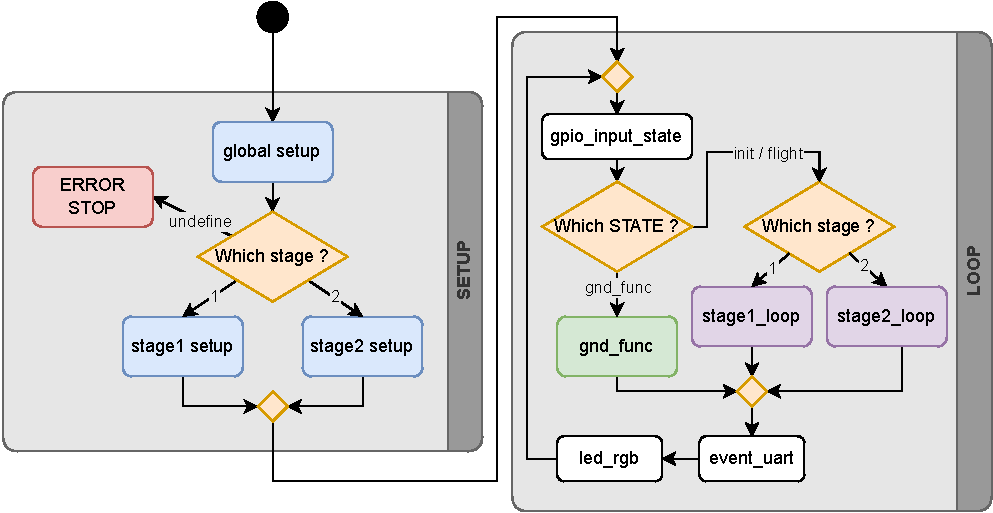
\includegraphics[width=0.9\textwidth]{figures/elec/main_sequenceur.drawio.pdf}
	\caption{Architecture générale du programme du séquenceur}
	\label{fig:main_sequenceur}
\end{figure}

Le programme se décompose en deux temps, visibles sur la figure. La fonction \texttt{setup()}, exécutée une seule fois à la
mise sous tension, réalise l'initialisation de la carte : configuration du matériel, puis détection de l'étage sur lequel elle
est installée, d'où découle l'initialisation des organes qui lui sont propres. La fonction \texttt{loop()} prend ensuite le
relais et s'exécute indéfiniment.\\

Ce firmware unique ne réalise pas une action unique. Il embarque un ensemble de sous-programmes, correspondant chacun à une
opération que la carte doit pouvoir exécuter, dont un seul s'exécute à la fois. C'est la boucle qui, à chaque itération, fait
progresser le sous-programme actif. Le choix de ce dernier revient à l'opérateur, au moyen du sélecteur de programme de
l'\acrshort{IHF}. Le schéma en distingue deux natures :

\begin{itemize}
	\item Les fonctions sol (\textit{gnd\_func}), en vert, regroupent les opérations de maintenance et de vérification employées
	pendant les campagnes de test et lors de l'assemblage. Chacune se termine d'elle-même et rend la main au séquenceur, qui se
	remet en attente d'une nouvelle consigne.
	\item Le programme de campagne de lancement (\textit{stage[1/2]\_loop}), en violet, correspond quant à lui au déroulement d'un
	lancement : une fois engagé, il ne rend jamais la main et enchaîne l'armement de la fusée puis son vol.
\end{itemize}

\paragraph*{Détection de l'étage} Le firmware étant commun aux deux cartes, celles-ci doivent pouvoir déterminer seules le rôle
qu'elles ont à tenir. Lors du montage de la fusée, un jumper peut être placé sur le séquenceur selon deux configurations
différentes, correspondant à l'étage sur lequel il est installé. Le programme lit cette configuration au démarrage. Si aucune des
deux états n'est détecté, du fait que le jumper n'est pas présent par exemple, la configuration est jugée invalide : la LED passe
au rouge et le programme s'arrête, plutôt que de laisser une carte s'exécuter sans savoir quel étage elle pilote. Si la LED est
clignote une fois en vert, alors le 1er étage est détecté, si elle est bleu, alors c'est le 2e étage qui est détecté.\\

Cette lecture, effectuée une seule fois, conditionne tout le reste de l'exécution. Elle détermine d'une part la fonction
d'initialisation appelée (\texttt{setup\_stage\_1} ou \texttt{setup\_stage\_2}), qui déclare les entrées utilisées par l'étage
et initialise ses actionneurs. Elle détermine d'autre part le contenu des fonctions sol : une même position du sélecteur ne
désigne pas la même opération selon l'étage, chacun ne disposant pas des mêmes organes.
 
\paragraph*{Structure de la boucle} La fonction \texttt{loop()} conserve une structure constante tout au long de l'exécution,
quel que soit le sous-programme actif. Elle se décompose en quatre étapes, décrites et illustrées ci-après :

\vspace{0.4cm}

\hspace*{-\parindent}%
\begin{minipage}{0.5\textwidth}
	\begin{lstlisting}[
		language=C,
		frame=tb,
		tabsize = 2,
		% showtabs=true,
		% tab = \smash{\rule[-.25\baselineskip]{.4pt}{\baselineskip}\kern0.9em}
	]
void loop() {
	update_gpio_input_states(...);

	switch (current_phase_type) {
		case STAGE_PHASE_GROUND_FUNC:
			...
			break;
		case STAGE_PHASE_INIT:
		case STAGE_PHASE_FLIGHT:
			switch (stage) {
				case ROCKET_FIRST_STAGE: {
					loop_stage_1(...);
					break;
				}
				case ROCKET_SECOND_STAGE: {
					loop_stage_2(...);
					break;
				}
				case ROCKET_STAGE_NO_SET: {
					// Wait what ????
				}
			}
			break;
	}

	event_uart_producer_run(...);

	LED_RGB_SetColor(...);
}
	\end{lstlisting}
\end{minipage}
\hfill
\begin{minipage}{0.45\textwidth}	
	\begin{itemize}
		\item \texttt{update\_gpio\_input\_states} relève l'état de l'ensemble des entrées électronique de la carte. Ce relevé
		groupé est préférable à une lecture de chaque broche au moment où une condition l'exige : toutes les décisions prises au
		cours d'une même itération s'appuient ainsi sur une image cohérente des entrées, prise à un instant unique, et une même
		broche ne peut pas être vue dans deux états différents par deux conditions successives. De plus, cela permet de mettre
		plus simplement en place un mécanisme de filtrage logiciel des entrées. Bien qu'il ne fut pas nécessaire pour le projet,
		cette fonctionnalité a été étudiée.\\

		\item L'aiguillage vers le sous-programme actif, qui distingue les fonctions sol (\texttt{STAGE\_PHASE\_GROUND\_FUNC}) du
		programme de campagne de lancement. Ce dernier se subdivise en deux phases, la phase d'initialisation en rampe
		(\texttt{STAGE\_PHASE\_INIT}) et le vol (\texttt{STAGE\_PHASE\_FLIGHT}), Cette distinction reste toutefois sans effet
		ici, puisque les deux cas conduisent à la même fonction, propre à l'étage, la logique de la phase étant gérée à
		l'intérieur de cette fonction.
	\end{itemize}
\end{minipage}

\vspace{0.4cm}

\begin{itemize}
	\item \texttt{event\_uart\_producer\_run} assure la transmission, vers l'expérience APEX, du journal des événements
	survenus dans le séquenceur. Son fonctionnement est détaillé en section \ref{subsec:log_apex}.\\

	\item \texttt{LED\_RGB\_SetColor} met à jour la LED de signalisation, unique retour d'information disponible sur la fusée une
	fois celle-ci refermée. (Plus de détails sur la gestion de la LED en section \ref{subsubsubsec:seq_leds}.)
\end{itemize}

\paragraph*{Une contrainte d'écriture} La boucle ne doit jamais être bloquée durablement, sous peine de retarder la
surveillance des événements de vol. Aucune opération longue ne peut donc y être écrite d'un seul tenant : chaque
sous-programme est réalisé sous forme de machine à états, dont l'état est conservé d'une itération à l'autre et qui progresse
d'au plus une transition par passage. Cette contrainte ne s'applique en revanche pas à \texttt{setup()}, qui s'exécute avant
toute échéance temporelle et peut donc attendre la fin d'une initialisation matérielle sans conséquence.

\newpage

\subsubsection{Sous-programmes}
\label{subsubsec:seq_sous_programmes}

La section précédente a décrit la structure du firmware et la manière dont il aiguille l'exécution vers l'un ou l'autre de ses
sous-programmes. Celle-ci en détaille le contenu, c'est-à-dire ce que le séquenceur exécute réellement.\\

Deux types de sous-programmes coexistent dans le firmware :
\begin{itemize}
	\item Les fonctions sol, d'une part, permettent de manipuler individuellement les organes de la fusée lors des essais et de
	l'assemblage. Chacune constitue une opération indépendante, déclenchée à la demande et répétable à volonté.
	\item Le programme de campagne de lancement, d'autre part, couvre le déroulement complet d'un lancement. Il constitue un
	sous-programme unique, mais se déroule en deux temps : une phase d'initialisation, qui amène la fusée à un état vérifié et
	prêt au décollage, puis une phase de vol, qui s'exécute sans aucune intervention possible.
\end{itemize}

\subsubsubsection{Fonctions sol}
\label{par:seq_ground_funcs}

De nombreuses opérations doivent pouvoir être commandées en dehors de tout vol : déployer les aérofreins pour vérifier leur
débattement, ouvrir et refermer une trappe de parachute, actionner le système de séparation lors de l'assemblage des deux
étages... Le séquenceur reste accessible et reprogrammable même fusée assemblée, mais recompiler et téléverser un firmware pour
chacune de ces manipulations serait fastidieux, et surtout risqué : la carte qui vole ne serait plus celle qui a été validée. Ces
opérations sont donc embarquées une fois pour toutes dans le firmware, sous forme de fonctions sol, et rendues accessibles
par leur numéro depuis l'\acrshort{IHF}.

\hspace*{-\parindent}%
\begin{minipage}{0.5\textwidth}
	\subparagraph*{Sélection et exécution} En l'absence de fonction sol active, le séquenceur attend un appui sur le bouton
	poussoir. La position du sélecteur n'est lue qu'à cet instant précis, et non en continu : manipuler le sélecteur ne déclenche
	donc rien tant que l'opérateur n'a pas validé son choix. La valeur lue détermine la suite : la position 0 engage le programme
	de campagne de lancement, tandis que les positions 1 à 15 sélectionnent la fonction sol correspondante, qui devient alors la
	fonction active. Le tableau \ref{tab:ground_funcs} récapitule les fonctions disponibles sur chaque étage.\\

	\subparagraph*{Contrat d'une fonction sol} Toutes les fonctions sol partagent la même signature et le même contrat. Appelées
	à chaque itération de la boucle tant qu'elles sont actives, elles renvoient \texttt{GROUND\_FUNC\_STATE\_RUNNING} pour
	signaler qu'elles n'ont pas terminé, ou \texttt{GROUND\_FUNC\_STATE\_DONE} pour rendre la main au séquenceur, qui se remet
	alors en attente d'une nouvelle consigne. Une opération de plusieurs secondes n'est donc jamais exécutée d'un seul tenant :
	elle conserve son avancement dans des variables persistantes et progresse d'un pas à chaque appel.
\end{minipage}
\hfill
\begin{minipage}{0.45\textwidth}
	\begin{figure}[H]
		\centering
		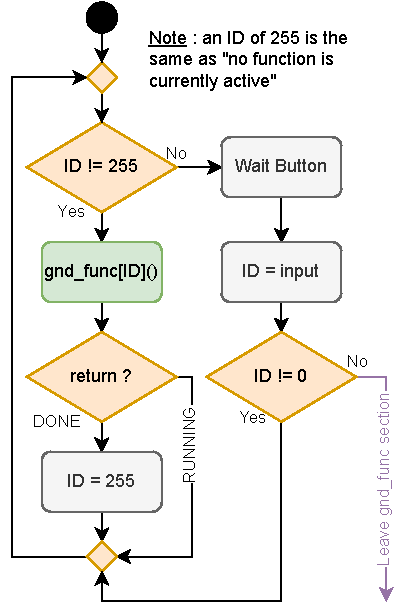
\includegraphics[width=0.9\textwidth]{figures/elec/Gnd_func.drawio.pdf}
		\caption{Sélection et exécution d'une fonction sol}
	\end{figure}
\end{minipage}

\newpage

\begin{table}[H]
    \centering
    \begin{tabular}{c l l}
        \hline
        \textbf{N\textsuperscript{o}} & \textbf{Nom} & \textbf{Description} \\
        \hline
        \multicolumn{3}{l}{\textit{Premier étage}} \\
        \hline
		0 & Programme de lancement & Déroulement complet d'une campagne de lancement \\
        1 & Référence aérofreins & Recherche de butée de l'actionneur d'aérofreins \\
        2 & Référence trappe & Recherche de butée de la trappe de parachute \\
        3 & Référence séparation & Recherche de butée du système de séparation \\
        4 & Man\oe uvre aérofreins & Déplacement d'une position à chaque appui \\
        5 & Man\oe uvre trappe & Déplacement d'une position à chaque appui \\
        6 & Man\oe uvre séparation & Déplacement d'une position à chaque appui \\
        7 à 15 & --- & Emplacements réservés \\
        \hline
        \multicolumn{3}{l}{\textit{Second étage}} \\
        \hline
		0 & Programme de lancement & Déroulement complet d'une campagne lancement \\
        1 & Référence trappe & Recherche de butée de la trappe de parachute \\
        2 & Man\oe uvre trappe & Déplacement d'une position à chaque appui \\
        3 & Validation attitude & Contrôle des conditions d'allumage et de la chaîne associée \\
        4 & Test allumage & Activation de la sortie d'allumage tant que la fonction est active \\
        5 à 15 & --- & Emplacements réservés \\
        \hline
    \end{tabular}
    \caption{Fonctions sol disponibles sur chaque étage}
    \label{tab:ground_funcs}
\end{table}

\vspace{-0.8cm}

\subparagraph*{Opérations sur les actionneurs} Les sous-programmes 1 à 6 pour le premier étage et 1 à 2 pour le second étage
commandent des actionneurs. Il existe deux types d'opérations sur ces organes : la mise en référence et la man\oe uvre :
\begin{itemize}
	\item La \emph{mise en référence} lance, au premier appel, la recherche d'une butée mécanique d'un actionneur et active un
	motif lumineux d'attente. Aux appels suivants, elle interroge l'avancement de l'opération et renvoie \texttt{RUNNING} tant
	que celle-ci n'est pas achevée. Dès que la butée est atteinte, c'est à dire que le servomoteur n'arrive plus à évoluer, la
	fonction renvoie \texttt{DONE}.
	\item La \emph{man\oe uvre} met en mouement un actionneur. Elle fait progresser le système mécanique auquel elle réfère d'une
	position vers une autre à chaque appui sur le bouton, en changeant de sens une fois la dernière (ou la première) position
	atteinte.
	% L'opérateur peut ainsi parcourir l'ensemble des positions d'un organe par appuis successifs, et vérifier visuellement son
	% débattement. La fonction refuse de s'exécuter si l'actionneur n'a pas été préalablement mis en référence, ses positions
	% n'ayant alors aucune signification.
\end{itemize}

Tous les systèmes mécaniques du projet SP-02 possèdent 3 positions distinctes, correspondant à des angles de rotation différents.
Le nombre 3 n'est pas une limite imposée, seulement une coincidence du besoin de chaque organe. Le tableau
\ref{tab:positions_actionneurs} ci-après récapitule les positions de chaque actionneur, ainsi que l'angle de rotation
correspondant :

\vspace{-0.1cm}

\begin{table}[H]
	\centering
	\begin{tabular}{ r r l }
		\hline
		\textbf{Position} & \textbf{Angle ($\degres$)} & \textbf{Description} \\
		\hline
		\multicolumn{3}{l}{\textit{Aérofreins}} \\
		\hline
		0 & 0	& Position fermée (maximale servant au démontage du système) \\
		1 & 30	& Position fermée (à fleur de la surface de la fusée) \\
		2 & 120 & Position ouverte \\
		\hline
		\multicolumn{3}{l}{\textit{Trappes (1er \& 2ème étage)}} \\
		\hline
		0 & 0	& Position verouillée \\
		1 & 45	& Position déverouillée \\
		2 & 90	& Position poussant la trappe pour forcer son ouverture \\
		\hline
		\multicolumn{3}{l}{\textit{Système de séparation}} \\
		\hline
		0 & 0	& Position verouillée \\
		1 & 590	& Position déverouillée \\
		2 & 740	& Position ressorts déclenchés \\
		\hline
	\end{tabular}
	\caption{Positions des actionneurs et angles de rotation correspondants}
	\label{tab:positions_actionneurs}
\end{table}

\newpage

% \noindent Pour la suite, nous prendrons l'exemple du système d'aérofrein.

\hspace*{-\parindent}%
\begin{minipage}{0.64\textwidth}
	Prendrons l'exemple du système d'aérofrein. Une opération sur un organe mécanique ne peut se faire que si ce dernier a
	préalablement été calibré via l'opération de \textit{mise en référence}. Pour la réaliser sur les aérofrein, l'opérateur
	doit sélectionner via l'\acrshort{IHF} le programme \texttt{1} puis appuyer sur le bouton \texttt{RUN}. La led se met alors
	à clignoter rapidement en jaune indiquant que l'opération est en cours. Le système peut se trouvé dans n'importe quelle des
	positions (qu'elle soit préalablement défini ou non), cette action le ramènera forcément dans la position 0
	(\ref{fig:positions_af:subfig:0}). Le clignotement de la led s'arrête lorsque l'opération se termine.\\

	Ensuite, pour passer d'une position à une autre, l'opérateur utilise le programme \texttt{2} (\textit{man\oe vre}). Il
	permet de jouer l'ensemble des positions. Les seules transition admisent sont celles entre deux positions adjacentes, soit :
	$0 \longleftrightarrow 1$ et $1 \longleftrightarrow 2$. Avec le programme \texttt{2} de sélectioné, à chaque appuie sur le
	bouton \texttt{RUN}, une transition est réalisé. Par exemple, en partant de la position 0 et en appuyant 5 fois sur le
	bouton, la séquence suivante est réalisée :
	$$0 \longrightarrow 1 \longrightarrow 2 \longrightarrow 1 \longrightarrow 0 \longrightarrow 1$$
	L'opérateur peut ainsi parcourir l'ensemble des positions d'un organe par appuis successifs, et vérifier visuellement son
	débattement.
\end{minipage}
\hfill
\begin{minipage}{0.32\textwidth}
	\vspace{-0.55cm}
	\begin{figure}[H]
		\centering
		\begin{subfigure}{\textwidth}
			\centering
			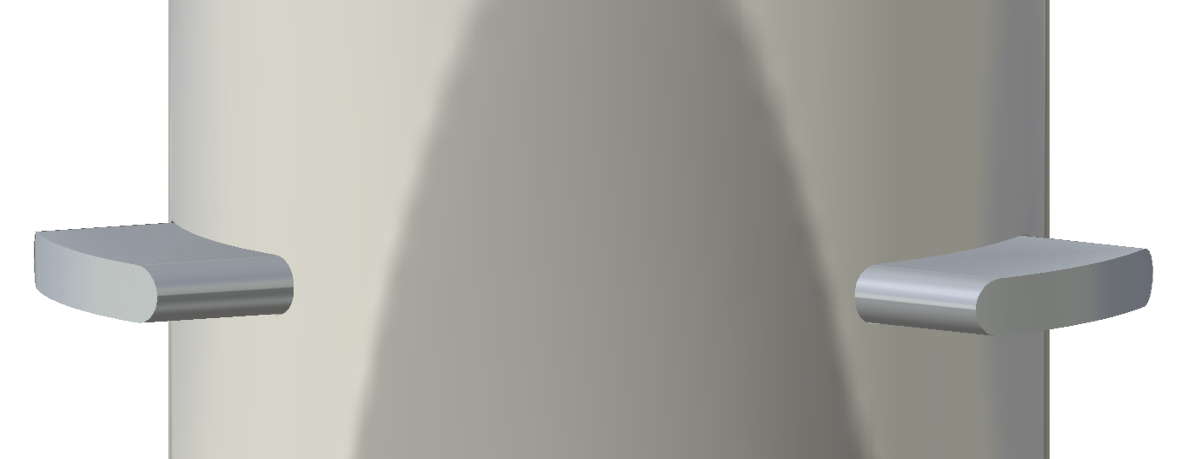
\includegraphics[width=\textwidth]{figures/elec/AF_2.png}
			\caption{Position 2}
			\label{fig:positions_af:subfig:2}
		\end{subfigure}
		\begin{subfigure}{\textwidth}
			\centering
			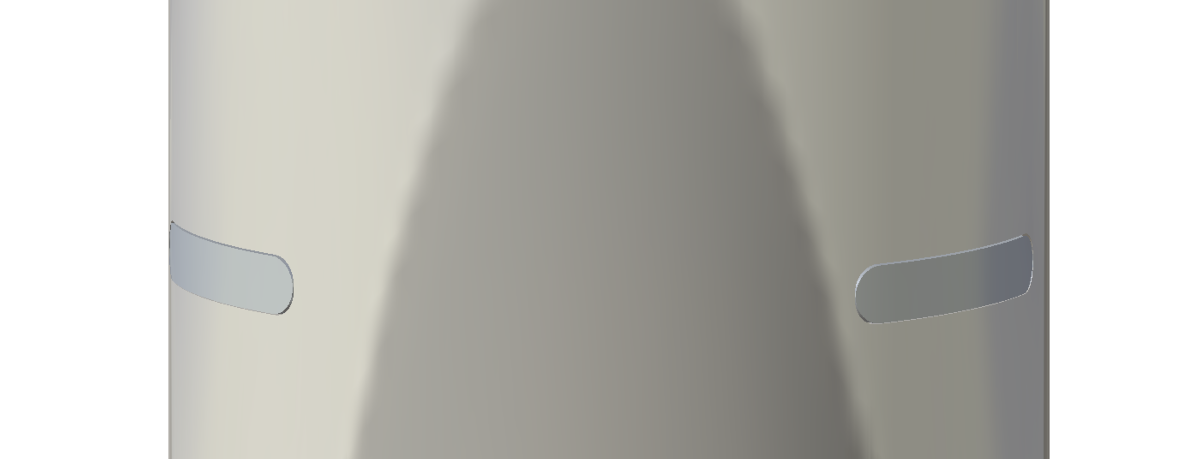
\includegraphics[width=\textwidth]{figures/elec/AF_1.png}
			\caption{Position 1}
			\label{fig:positions_af:subfig:1}
		\end{subfigure}
		\begin{subfigure}{\textwidth}
			\centering
			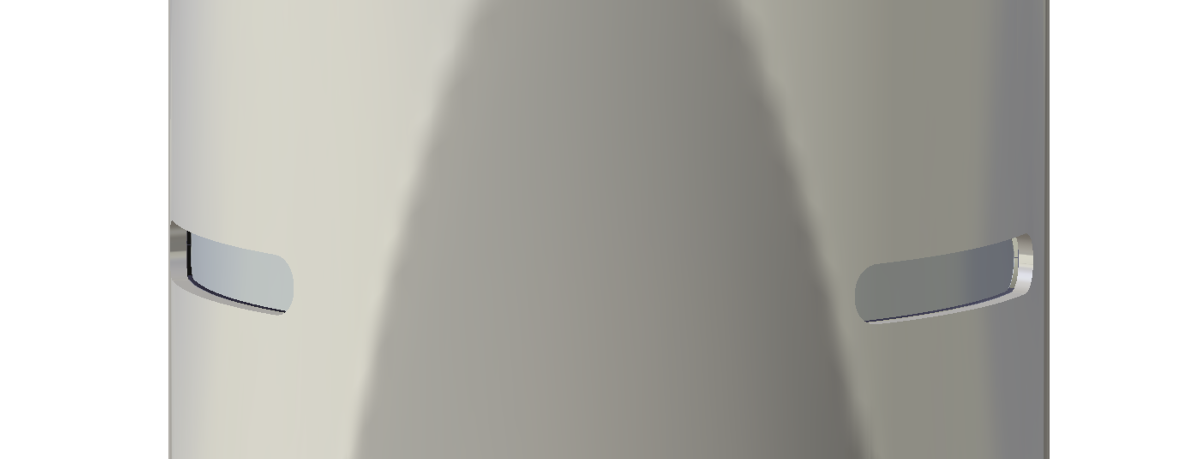
\includegraphics[width=\textwidth]{figures/elec/AF_0.png}
			\caption{Position 0}
			\label{fig:positions_af:subfig:0}
		\end{subfigure}
		\caption{Les 3 positions du système d'aérofrein}
		\label{fig:positions_af}
	\end{figure}
\end{minipage}
\hfill\hfill

\vspace{0.2cm}

\noindent Un autre exemple qui est intéressant d'étudier est la procédure pour coupler les étages après la mise sous tension du
premier étage et hors du programme de vol (programme \texttt{0}). Toutes opérations s'effectue sur le premier étage :
\begin{enumerate}
	\item Vérifier visuellement qu'aucun objet ne gêne le système mécanique de séparation. 
	\item Choisir le programme \texttt{3} et le lancer en appuyant sur le bouton afin de réaliser la mise en référence du
	système.
	\item Choisir le programme \texttt{6} et le lancer 3 fois en attendant que le servomoteur ait fini d'atteindre sa position
	à chaque itération. Le système a alors effectué la séquence suivante $0 \longrightarrow 1 \longrightarrow 2 \longrightarrow 1$
	\item Armer les ressorts du système.
	\item Assembler les étages et s'assurer que le jeu entre les étages est suffisament faible pour permettre le verouillage.
	\item Lancer une 4ème fois le programme \texttt{6}. Cela ramènera le système à la position 0 et verouillera les étages.
\end{enumerate}

Tout ce système d'opération réalisable sur les actionneur est rendu possible grâce aux outils logiciels présenté en section
\ref{subsubsubsec:seq_actionneurs}.

\vfill

\subparagraph*{Fonctions liées à l'allumage} La position 3 du deuxième étage valide la condition qui autorisera l'allumage du
propulseur en vol. Cette fonction acquiert en continu les mesures de la centrale inertielle, en déduit l'élévation et l'azimut
de la fusée, puis les compare aux valeurs attendues au moment de l'allumage. Le résultat est restitué par la couleur de la LED :
\begin{itemize}
	\item verte si les deux angles sont dans leur tolérance ;
	\item bleue si un seul l'est ;
	\item rouge sinon.
\end{itemize}
La sortie d'allumage est pilotée en conséquence, ce qui permet de valider la chaîne complète, depuis la mesure d'attitude jusqu'à
la commande. Les grandeurs calculées sont par ailleurs émises sur la liaison \acrshort{USB}, afin de pouvoir être tracées et
vérifiées finement en atelier. L'opérateur bascule entre les modes (accélération et gyromètre) et quitte la fonction par des
appuis courts ou longs sur le bouton. Plus d'informations sur la mesure d'attitude sont disponibles en section
\ref{subsec:mesure_attitude}.\\

La position 4 est plus directe : elle maintient l'ordre d'allumage du propulseur du 2e étage active tant que la fonction
s'exécute, et la désactive au moment d'en sortir. Elle permet de vérifier la continuité de la chaîne pyrotechnique indépendamment
de toute condition d'attitude. Ces deux fonctions ne sont évidemment employées qu'avec un dispositif de mesure en lieu et place
de l'allumeur.

\newpage

\subsubsubsection{Phase d'initialisation}
\label{subsubsec:seq_initialisation}

Sélectionner le programme \texttt{0} engage le programme de campagne de lancement, qui s'ouvre sur une phase d'initialisation.
Son rôle est d'amener la fusée, depuis un état quelconque, jusqu'à un état vérifié et prêt au décollage. Elle se distingue des
fonctions sol sur un point essentiel : l'opérateur n'y choisit plus ce qu'il exécute. Le séquenceur impose un ordre, valide chaque
étape avant de passer à la suivante, et refuse d'avancer tant que les conditions ne sont pas réunies. La procédure de préparation
est ainsi rendue obligatoire par le logiciel, plutôt que confiée à la rigueur de l'opérateur.

\subparagraph*{Une progression validée pas à pas} La phase se déroule comme une succession d'étapes séparées par des attentes
d'appui sur le bouton. Ce découpage répond à une règle que s'est fixée l'équipe : aucun servomoteur ne doit jamais être mis en
mouvement automatiquement. Toute commande d'actionneur est précédée d'une validation explicite de l'opérateur, qui s'assure au
préalable que rien n'entrave la course du système concerné.\\

Les étapes s'enchaînent dans l'ordre suivant sur le premier étage, représenté sur la figure \ref{fig:init_stage_1} : attente de
l'insertion du \texttt{JACK READY}, puis mise en référence successive des aérofreins, de la trappe de parachute et du système de
séparation, et enfin vérification globale de l'état de la fusée. Le second étage suit la même trame, réduite aux organes dont
il dispose : \texttt{JACK READY}, mise en référence de sa trappe, puis vérification globale (\ref{fig:init_stage_2}).

\begin{figure}[H]
    \centering
    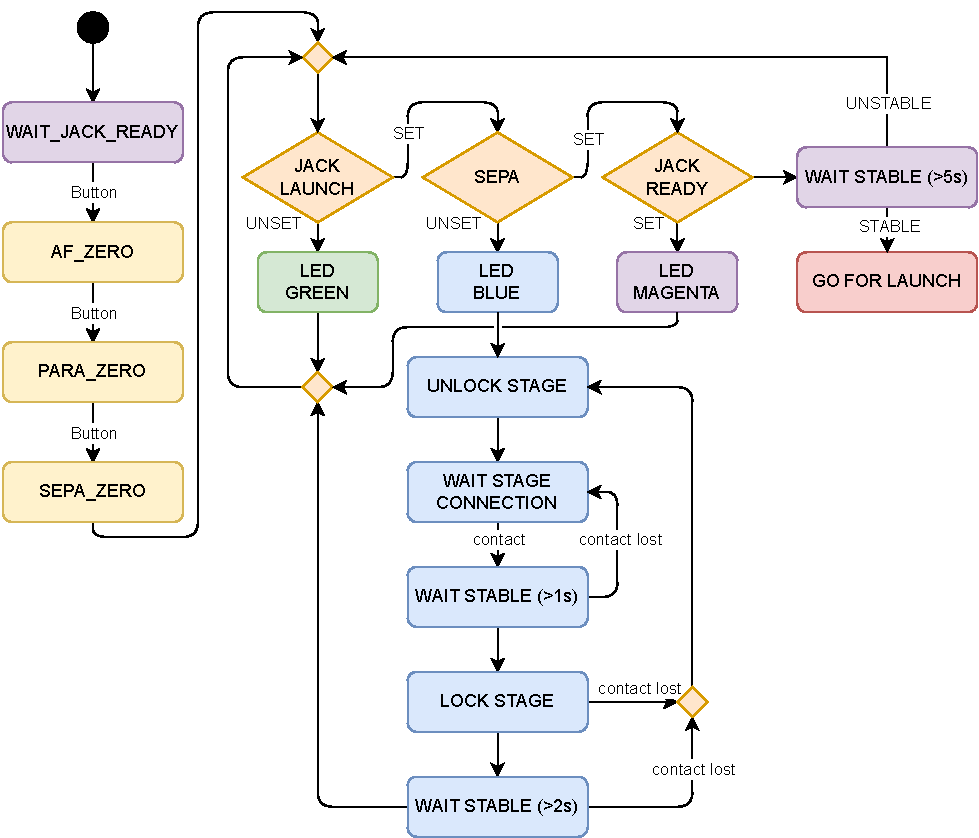
\includegraphics[width=\textwidth]{figures/elec/sequenceur_stage_1_init.drawio.pdf}
    \caption{Phase d'initialisation du premier étage.}
    \label{fig:init_stage_1}
\end{figure}

\newpage

\subparagraph*{La vérification globale} Une fois les actionneurs mis en référence, la fusée entre dans une boucle de
surveillance. L'opérateur n'y déclenche plus d'étape : le séquenceur évalue désormais de lui-même les conditions nécessaires au
départ, et pilote au passage l'assemblage des étages décrit plus loin. Deux de ces conditions portent sur la configuration
mécanique de la fusée : le \texttt{JACK\_LAUNCH} doit être inséré, et les deux étages doivent être assemblés avec le mécanisme
de séparation verrouillé. La troisième, le retrait du \texttt{JACK\_READY}, n'est évaluée qu'une fois les deux premières
satisfaites.\\
 
La figure \ref{fig:init_stage_1} présente ces vérifications sous forme d'une chaîne de tests, mais il faut se garder de la lire
comme une progression figée : l'ensemble du cycle est reparcouru à chaque itération de la boucle principale. Les conditions sont
donc réévaluées en permanence, et rien n'est acquis une fois pour toutes. Si les étages sont désolidarisés après avoir été
assemblés, ou si le \texttt{JACK\_LAUNCH} est retiré, la condition correspondante redevient insatisfaite et la fusée recule
d'autant : c'est l'état courant du système qui compte, et non l'historique des étapes franchies.\\
 
Le \texttt{JACK\_READY} est arraché par les derniers opérateurs quittant le pas de tir, rampe déjà érigée. Tant qu'il est en
place, le séquenceur ne peut en aucun cas interpréter un faux contact ou une secousse liée aux manipulations comme un décollage,
et donc engager sa séquence de vol, ce qui conduirait, sur le second étage, à l'allumage du propulseur alors que des personnes
se trouvent à proximité immédiate. Son retrait constitue par ailleurs le signal de départ de la chaîne de télémesure de
l'expérience APEX. C'est pourquoi sa présence est exigée en début de séquence, et son retrait demandé en toute fin.

\hspace*{-\parindent}%
\begin{minipage}{0.55\textwidth}
\subparagraph*{L'assemblage des étages} La partie bleu de la figure détaille la séquence d'assemblage. Le premier étage,
seul sur la rampe, déverrouille son mécanisme de séparation puis attend le couplage du second étage. Dès que le contact est
détecté et maintenu pendant une seconde, il commande le verrouillage, puis vérifie pendant deux secondes supplémentaires que ce
contact reste établi avant de considérer l'assemblage abouti. Toute perte de contact fait reculer la séquence à l'étape
correspondante.\\
 
L'assemblage est ainsi entièrement automatique : les opérateurs n'ont qu'à emboîter les deux étages, le séquenceur se chargeant
du reste sans qu'aucune commande ne lui soit adressée. Si le contact est perdu, alors le séquenceur déverrouille le mécanisme de
séparation pour permettre un retour à un état pouvant accueillir le deuxième étage. La double temporisation écarte par ailleurs
les détections fugitives, fréquentes lors d'un emboîtement mécanique : une prise de contact intermittente pendant l'ajustement ne
déclenche pas de verrouillage prématuré.\\
\end{minipage}
\hfill
\begin{minipage}{0.35\textwidth}
	\begin{figure}[H]
		\centering
		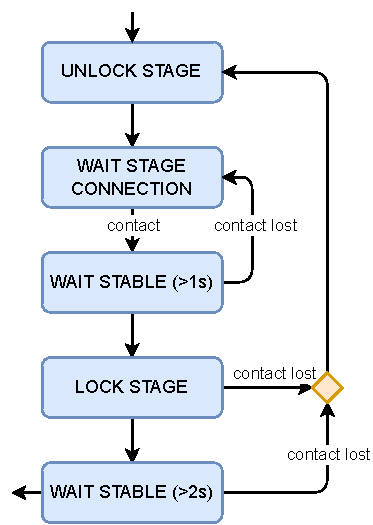
\includegraphics[width=\textwidth]{figures/elec/sequenceur_stage1_init_sepa_zoom.drawio.pdf}
		\caption{Zoom sur la séquence d'assemblage des étages.}
		\label{fig:init_stage_1_sepa_zoom}
	\end{figure}
\end{minipage}
\hfill
\hfill

\vspace{0.4cm}
 
Enfin, une action volontaire reste accessible à l'opérateur pendant toute la durée de cet état, bien qu'elle ne figure pas sur
la figure \ref{fig:init_stage_1} pour ne pas en alourdir la lecture : la commande de déverrouillage du mécanisme de
séparation. En sélectionnant la position correspondante du sélecteur et en appuyant sur le bouton, l'opérateur provoque le
déverrouillage puis, après une temporisation, le retour à l'état de vérification, la machine d'assemblage étant réinitialisée à
son premier état. Cette possibilité est nécessaire : elle permet de reprendre un assemblage qui s'avérerait incorrect sans avoir
à couper l'alimentation du séquenceur ni à revenir aux \textit{ground functions}, désormais inaccessibles.

\subparagraph*{La stabilisation finale} Lorsque toutes les conditions (\texttt{JACK\_LAUNCH}, assemblage des étages et
\texttt{JACK\_READY}) sont réunies, la fusée entre dans un dernier état d'attente, qui exige que cette situation soit
maintenue pendant cinq secondes. Toute rupture d'une condition durant ce délai ramène immédiatement à la boucle de
surveillance.

\newpage

La figure \ref{fig:init_stage_2} illustre la phase d'initialisation du second étage, qui ne diffère de celle du premier que par
la liste des actionneurs à mettre en référence et par l'absence de séquence d'assemblage. Bien que cet étage ne possède pas de
\texttt{JACK\_LAUNCH}, la condition correspondante est tout de même évaluée. Lorsque les deux étages sont assemblés, l'action de
brancher et débrancher le \texttt{JACK\_LAUNCH} sur le premier étage se voit répercutée sur le second. Retirer le
\texttt{JACK\_LAUNCH} du premier étage a pour effet d'allumer la led verte sur les deux étages, le brancher de nouveau les
éteint.

\begin{figure}[H]
    \centering
    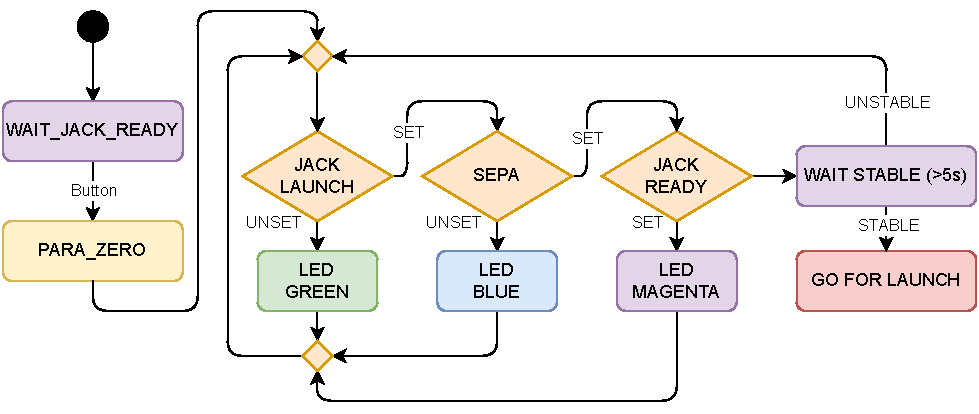
\includegraphics[width=\textwidth]{figures/elec/sequenceur_stage_2_init.drawio.pdf}
    \caption{Phase d'initialisation du deuxième étage.}
    \label{fig:init_stage_2}
\end{figure}

Cette étape d'initialisation de la fusée est conçue pour être vécue par l'opérateur plutôt que pour être franchie rapidement.
Chaque condition non satisfaite active son propre motif lumineux, dont la couleur identifie ce qui manque : vert pour le
\texttt{JACK\_LAUNCH}, bleu pour l'assemblage des étages, magenta pour le \texttt{JACK\_READY}. Le jaune, employé lors des
étapes précédentes, signale quant à lui une opération d'actionneur en cours. D'un simple coup d'\oe il, et sans instrument,
l'opérateur sait donc ce que le séquenceur attend de lui : une LED verte signifie que le \texttt{JACK\_LAUNCH} n'est pas inséré
alors qu'il devrait l'être, etc. Les figures \ref{fig:ramp_jack_ready_1} à \ref{fig:ramp_ready_to_fly} illustrent cette séquence
d'initialisation, avec les motifs lumineux correspondants.\\

À la mise sous tension, les deux étages reposent séparément sur la rampe. Chacun attend l'insertion de son
\texttt{JACK\_READY} et l'annonce par un motif magenta.

\begin{figure}[H]
    \centering
    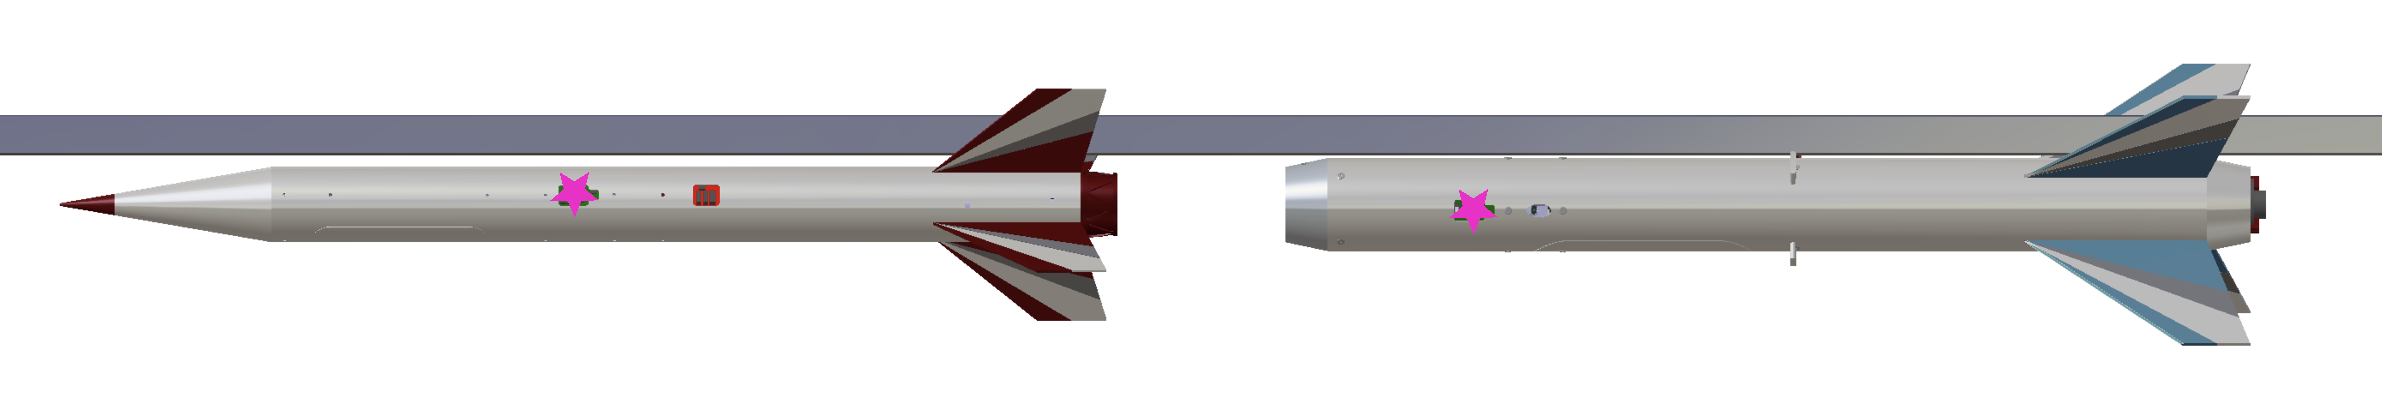
\includegraphics[width=\textwidth, height=0.15\textheight]{figures/elec/SP02_ramp_1.png}
    \caption{Etages non assemblés en rampe, indicateurs magenta sur les deux étages.}
    \label{fig:ramp_jack_ready_1}
\end{figure}

Les jacks insérés, l'opérateur valide successivement la mise en référence de chaque actionneur. Le motif jaune signale
l'opération en cours : trois étapes sur le premier étage, une seule sur le second.

\begin{figure}[H]
    \centering
    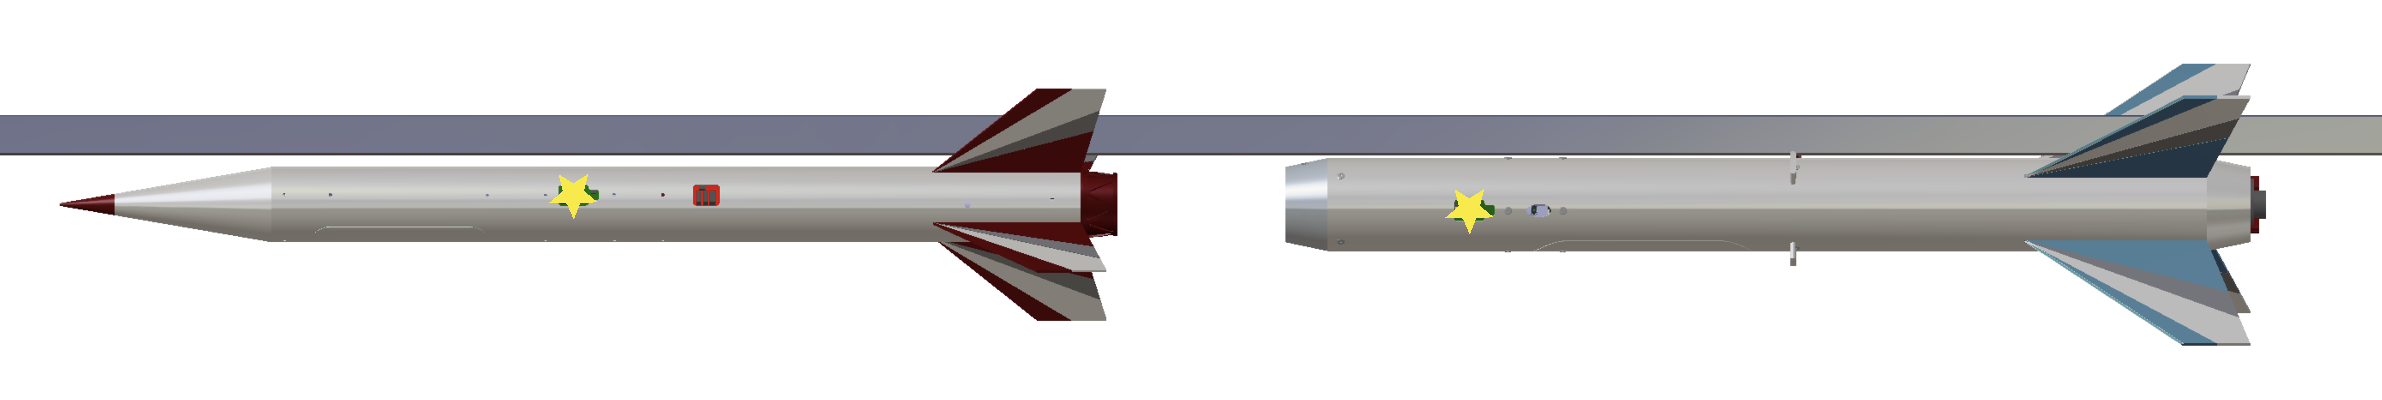
\includegraphics[width=\textwidth, height=0.15\textheight]{figures/elec/SP02_ramp_2.png}
    \caption{Etages non assemblés en rampe, indicateurs jaunes sur les deux étages.}
    \label{fig:ramp_actuators}
\end{figure}

Les actionneurs référencés, les deux étages entrent dans leur boucle de surveillance. Il leur manque alors les deux mêmes
conditions : le \texttt{JACK\_LAUNCH} n'est pas inséré et les étages ne sont pas assemblés. Les motifs vert et bleu alternent
donc sur les deux cartes.

\begin{figure}[H]
    \centering
    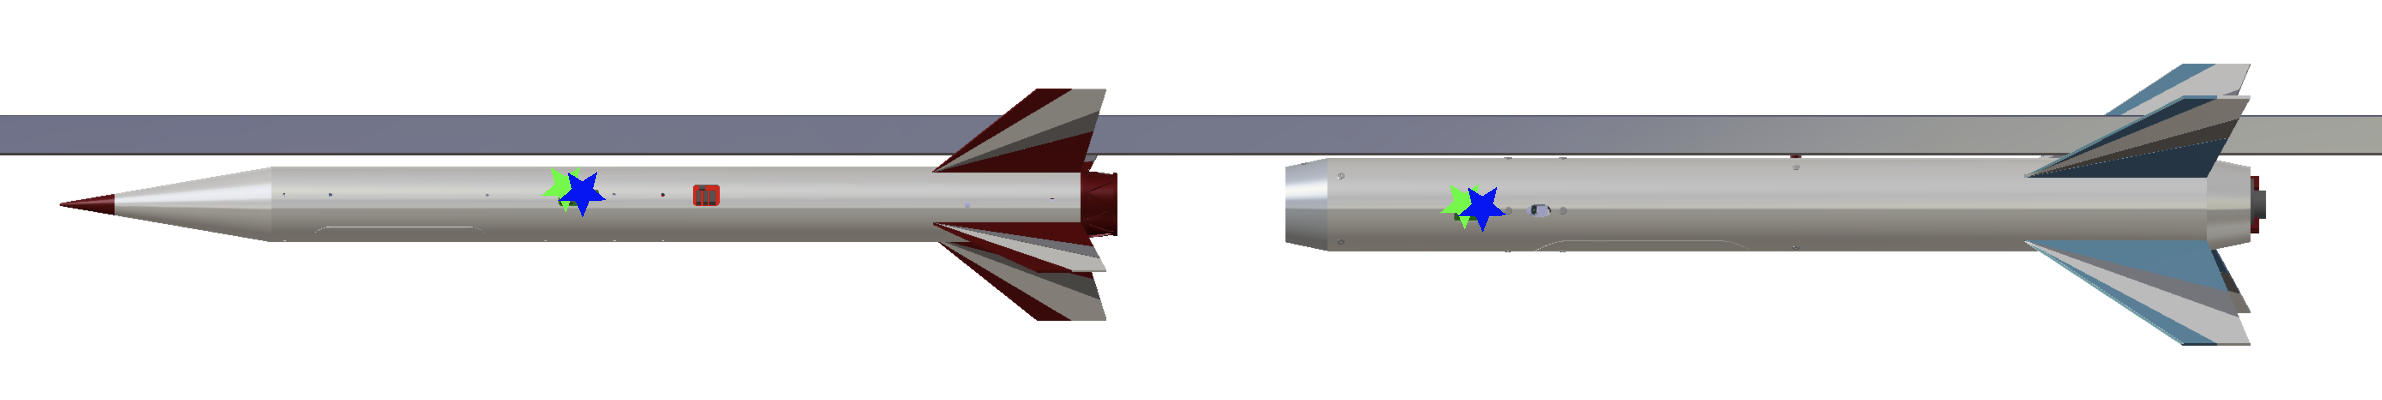
\includegraphics[width=\textwidth, height=0.15\textheight]{figures/elec/SP02_ramp_3.png}
    \caption{Etages non assemblés en rampe, indicateurs verts et bleus sur les deux étages.}
    \label{fig:ramp_jack_launch}
\end{figure}

L'insertion du \texttt{JACK\_LAUNCH} sur le premier étage éteint son motif vert. Le second étage, encore désolidarisé,
continue en revanche de l'afficher : le signal ne lui parvient que par le couplage mécanique, qui n'est pas encore établi. Les
deux étages n'affichent donc temporairement pas la même chose, ce qui est attendu.

\begin{figure}[H]
    \centering
    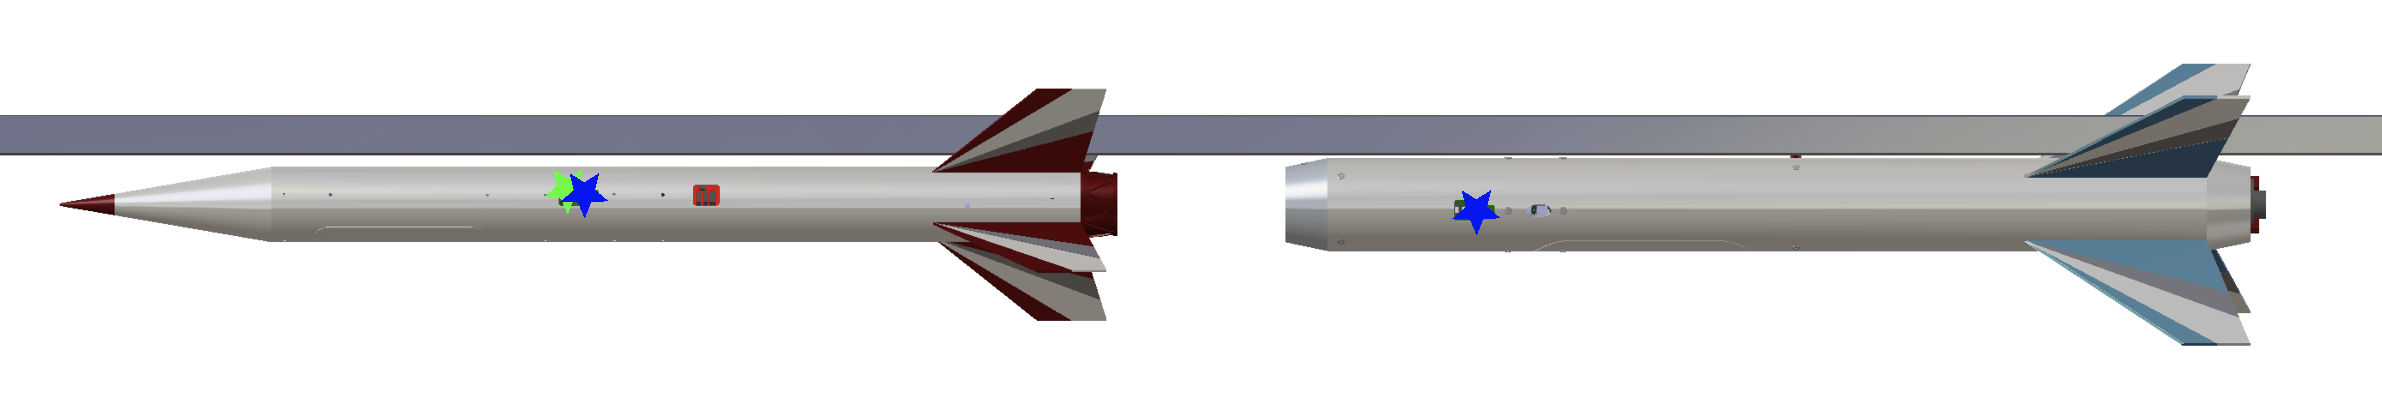
\includegraphics[width=\textwidth, height=0.15\textheight]{figures/elec/SP02_ramp_4.png}
    \caption{Etages non assemblés en rampe, indicateurs bleus sur les deux étages, vert également sur le 2e étage.}
    \label{fig:ramp_sepa}
\end{figure}

Les opérateurs emboîtent alors les deux étages. Le premier détecte le contact, le confirme et commande le verrouillage : les
motifs bleus s'éteignent de part et d'autre. Le second étage reçoit du même coup l'état du \texttt{JACK\_LAUNCH} et éteint son
motif vert. Ne subsiste que le magenta, qui réclame cette fois le retrait du \texttt{JACK\_READY}, dernier geste avant
l'évacuation du pas de tir.

\begin{figure}[H]
    \centering
    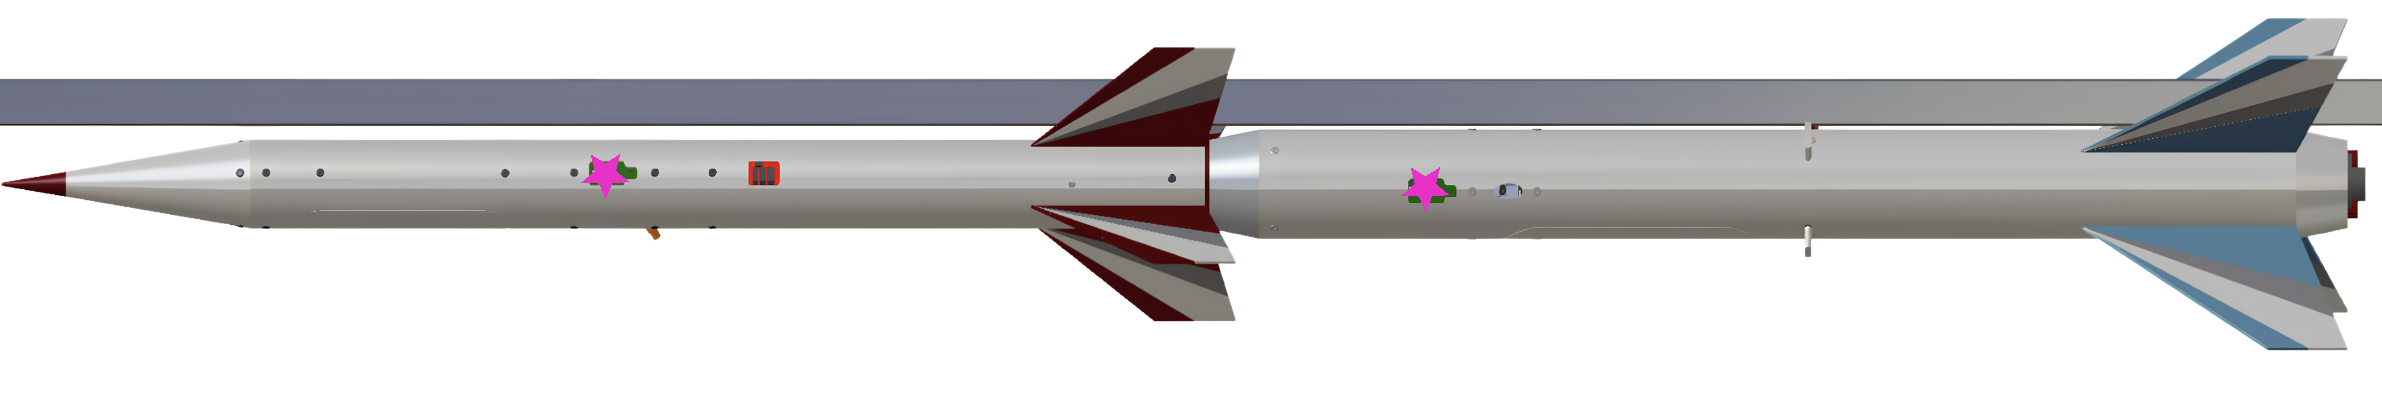
\includegraphics[width=\textwidth, height=0.15\textheight]{figures/elec/SP02_ramp_5.png}
    \caption{Etages assemblés en rampe, indicateur magenta sur les deux étages.}
    \label{fig:ramp_jack_ready_2}
\end{figure}

Les \texttt{JACK\_READY} retirés et l'ensemble des conditions maintenues pendant cinq secondes, les deux étages basculent en
phase de vol et l'annoncent par un motif rouge. La fusée est prête au décollage.

\begin{figure}[H]
    \centering
    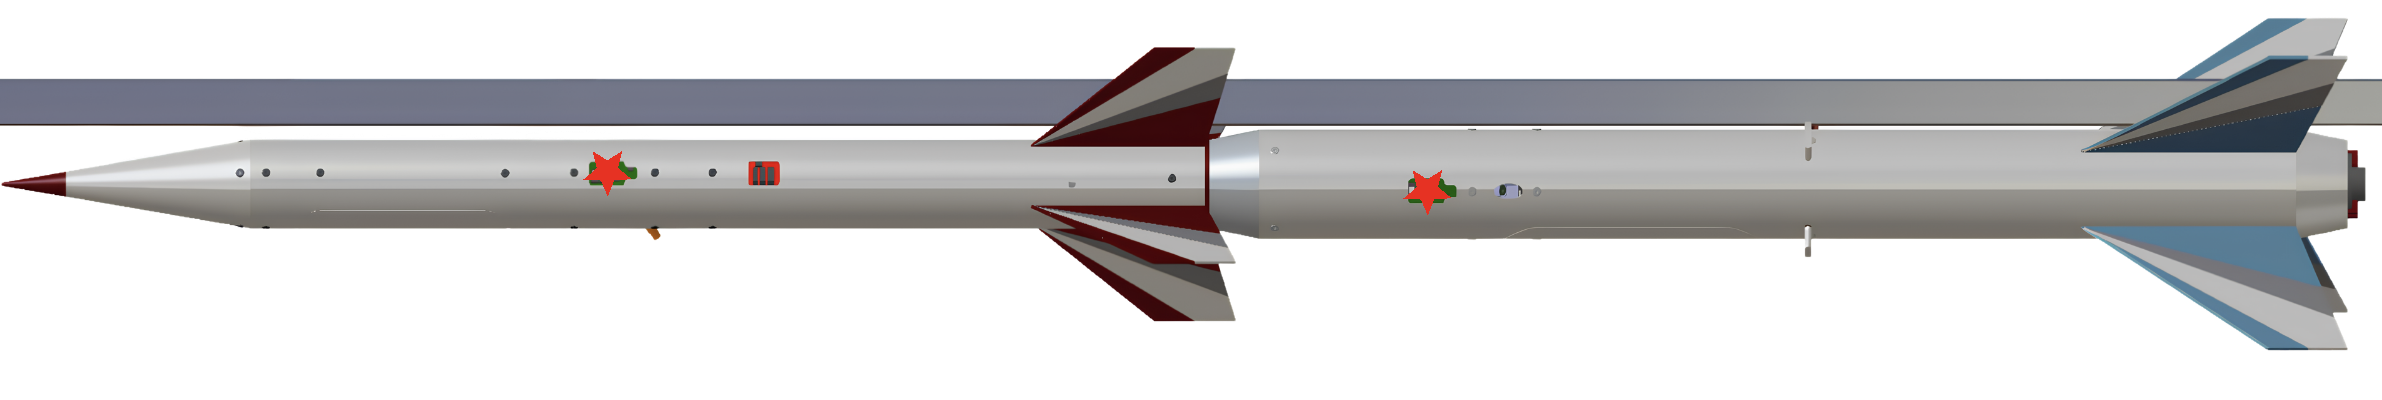
\includegraphics[width=\textwidth, height=0.15\textheight]{figures/elec/SP02_ramp_6.png}
    \caption{Etages assemblés en rampe, indicateur rouge sur les deux étages.}
    \label{fig:ramp_ready_to_fly}
\end{figure}

\newpage

\subsubsubsection{Phase de vol}
\label{subsubsec:seq_flight}

\subsubsection{Phase de vol}

La phase de vol constitue la dernière phase du programme de vol. Elle est atteinte à l'issue de la phase d'initialisation et
exécute la séquence des événements de vol jusqu'à l'ouverture de la trappe à parachute. L'ensemble des instants qui la
composent est défini relativement à $T_0$, l'instant du décollage, déterminé par l'arrachage du \texttt{JACK\_LAUNCH}.\\

La séquence est construite à partir de deux briques élémentaires, représentées sur la figure~\ref{fig:briques_sequence}. La\\
temporisation, notée $\mathrm{Wait}(T_x)$, maintient l'état courant tant que l'instant $T_x$ n'est pas atteint, puis exécute
l'action qui lui est associée. La fenêtre de détection, notée $\left\{T_x, \Delta T_x\right\}$ où $T_x$ désigne l'instant
d'ouverture de la fenêtre et $\Delta T_x$ sa durée, teste une condition physique et possède trois issues : le maintien dans
l'état tant que la condition n'est pas vérifiée, la confirmation lorsqu'elle l'est à l'intérieur de la fenêtre, et l'expiration
au-delà de $T_x + \Delta T_x$.\\

Les deux bornes de la fenêtre remplissent des rôles distincts. La borne inférieure écarte les détections prématurées : une
condition vérifiée avant $T_x$ ne peut correspondre à l'événement attendu. La borne supérieure garantit la progression de la
séquence en l'absence de détection, en orientant le programme vers une branche dégradée plutôt qu'en le laissant en attente
d'un événement qui ne surviendra pas.

\vfill

\begin{figure}[H]
	\centering
	\begin{subfigure}{0.8\linewidth}
		\centering
		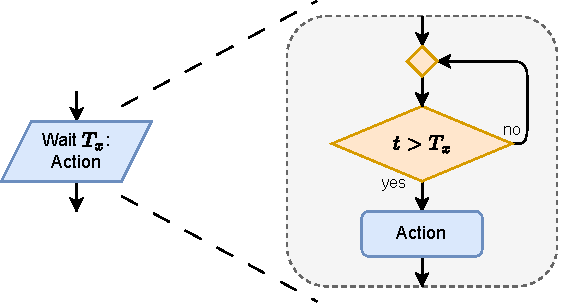
\includegraphics[width=\linewidth]{figures/elec/WAIT.drawio.pdf}
		\caption{Temporisation}
		\label{fig:brique_wait}
	\end{subfigure}
	\vspace{0.2cm}
	\begin{subfigure}{0.8\linewidth}
		\centering
		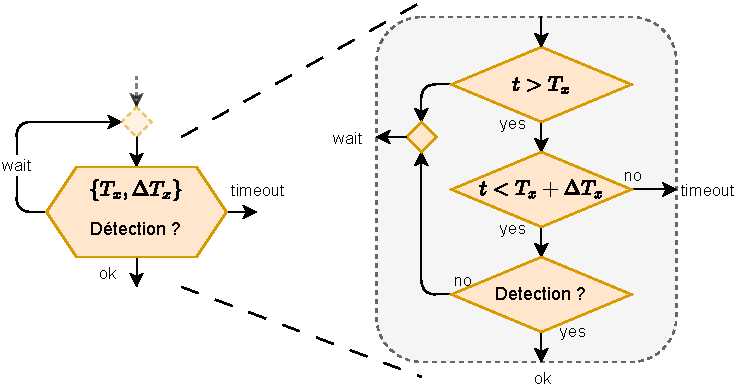
\includegraphics[width=\linewidth]{figures/elec/FT.drawio.pdf}
		\caption{Fenêtre de détection}
		\label{fig:brique_ft}
	\end{subfigure}
	\caption{Briques élémentaires de la séquence de vol et leur notation compacte}
	\label{fig:briques_sequence}
\end{figure}

\newpage

Les séquences de vol des deux étages sont représentées sur la figure~\ref{fig:sequences_vol}. Construites à partir des deux
briques précédentes, chaque étage exécute la séquence qui lui est propre : le 1er étage enchaîne les commandes du système de
séparation et des aérofreins, tandis que le 2e étage subordonne l'allumage de son moteur à la confirmation de la séparation
puis à la vérification de son attitude, selon la fenêtre d'attitude autorisée.\\

Les issues des fenêtres de détection déterminent le chemin suivi dans la séquence. Chacun de ces chemins correspond à un
scénario de vol, auquel est associée une fenêtre de détection de l'apogée qui lui est propre.

\begin{figure}[H]
    \centering
    \begin{subfigure}{0.48\linewidth}
        \centering
        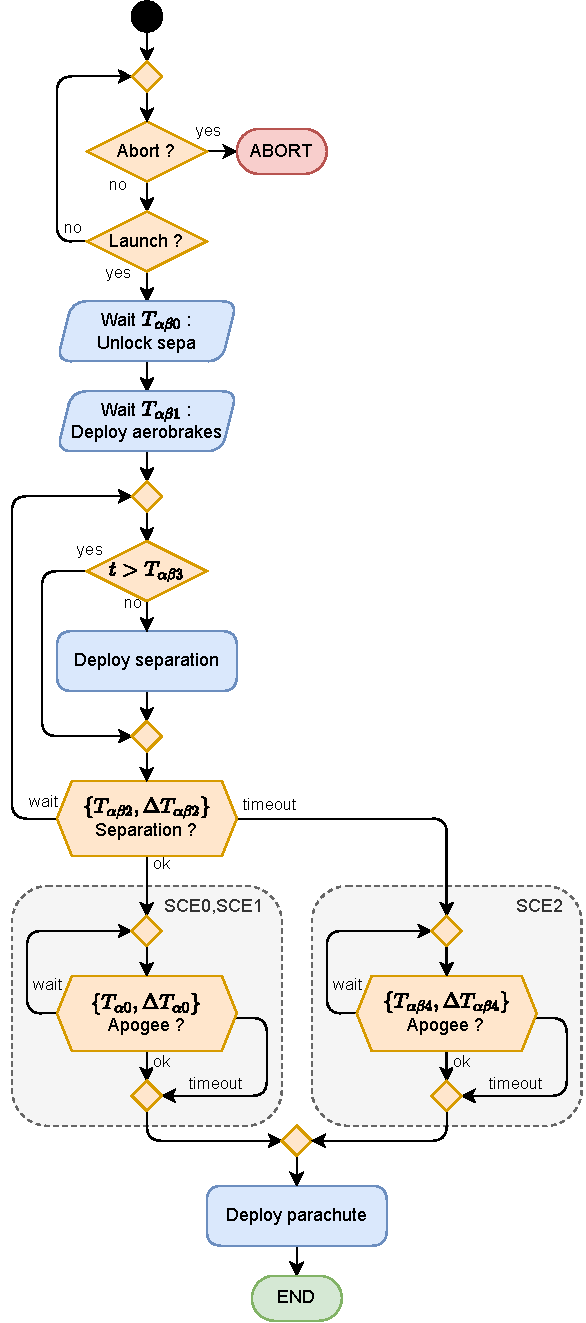
\includegraphics[width=\linewidth]{figures/elec/sequ1.drawio.pdf}
        \caption{1er étage}
    \end{subfigure}
    \hfill
    \begin{subfigure}{0.48\linewidth}
        \centering
        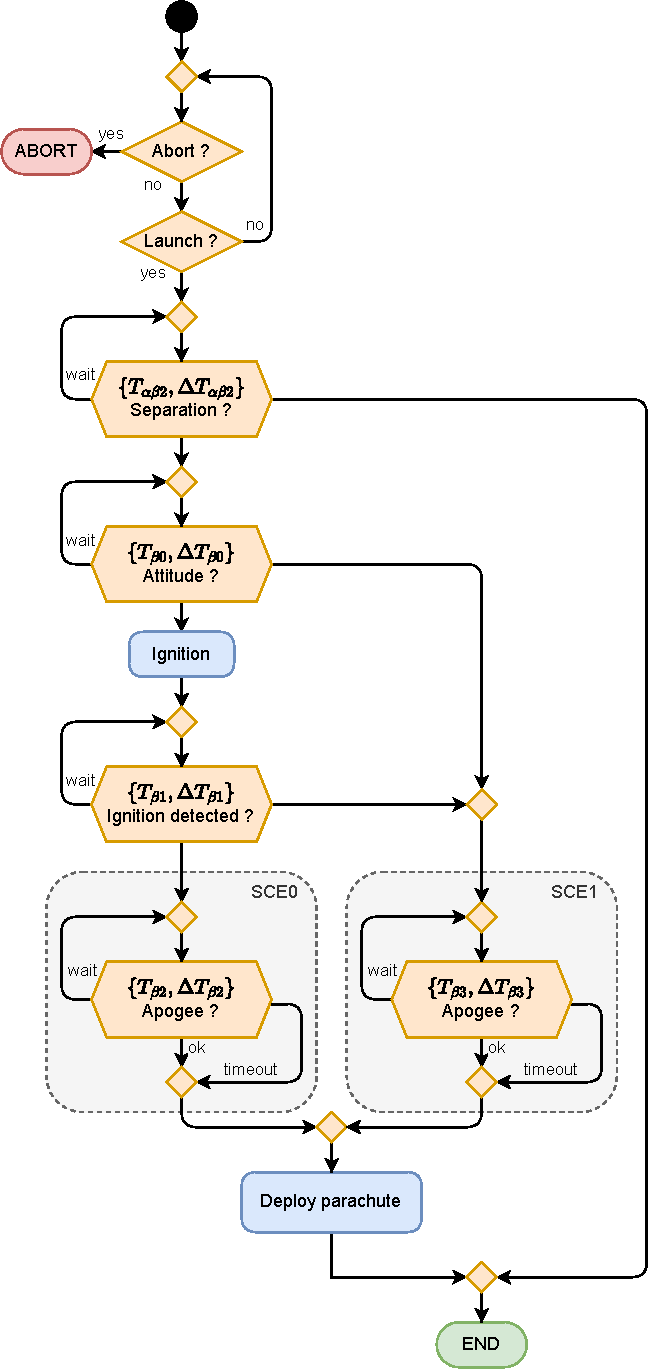
\includegraphics[width=\linewidth]{figures/elec/sequ2.drawio.pdf}
        \caption{2e étage}
    \end{subfigure}
    \caption{Schémas fonctionnels des séquenceurs des deux étages}
\end{figure}

\newpage

\subsubsection{Calcul d'attitude}
\label{subsec:mesure_attitude}

Afin de réaliser la mission, le séquenceur doit être capable de calculer l'attitude de la fusée à partir des mesures issues d'une
centrale inertielle. La construction de l'ordre de décision d'allumage du propulseur du second étage se découpe en 4 étapes
principales :

\begin{enumerate}
	\item Acquisition des mesures de la centrale inertielle \texttt{WT901B}.
	\item Filtrage des mesures pour réduire le bruit et les erreurs de mesure.
	\item Calcul de l'attitude de la fusée à partir des mesures filtrées.
	\item Comparaison de l'attitude calculée avec les valeurs attendues pour déterminer si l'allumage du propulseur est autorisé.
\end{enumerate}

\subsubsubsection{Acquisition des mesures et filtrage}

L'acquisition des mesures de la centrale inertielle est réalisée par le séquenceur via une liaison série \texttt{UART} full-duplex.
La \texttt{WT901B} est capable de fournir des mesures brutes d'accélération, de vitesse angulaire et de champ magnétique, ainsi que
des mesures d'attitude calculées par la centrale elle-même sous forme d'angle d'Euler et de quaternion.\\

Cependant, une incertitude sur les méthodes de calcul utilisées par la centrale et sur les paramètres de calibration de celle-ci
ont conduit les équipes du projet à ne pas se fier à ces mesures d'attitude. Bien qu'il est écrit que la \texttt{WT901B} est
capable de fournir des données cohérente en milieu dynamique, le risque que la forte poussée générée par le propulseur lors du
décollage puis la décélération brutale lors de l'extinction de celui-ci fausse les mesures d'attitude est trop important. En
effet, ce genre d'algorithme de calcul se sert de l'accélération pour corriger la dérive des gyromètres en considérant que le
module se trouve sous l'effet de la gravité terrestre seul.\\

Après avoir effectué des tests, il a été constaté que les simples mesures brutes des vitesses angulaires pouvaient suffire à
la détermination de l'attitude de la fusée. Cette méthode est sujette à une dérive, mais cette dernière est suffisamment faible
sur la durée du vol pour que l'attitude calculée reste cohérente. La chaine de calcul sera également connu et maitrisée par les
équipes du projet, ce qui permet de s'assurer de la cohérence des résultats.\\

La chaine d'aqcuisition et de filtrage utilise 3 bibliothèques logicielles développées pour le projet :
\begin{itemize}
	\item le pilote \texttt{wt901b} qui implémente le protocole série de la centrale inertielle ;
	\item l'utilitaire \texttt{data\_topic} qui permet de gérer les données acquises et de les rendre accessibles à d'autres
	parties du 	programme via un système de publication/abonnement ;
	\item l'utilitaire \texttt{iir\_filter} qui permet de filtrer les données pour réduire le bruit et les erreurs de mesure.\\
\end{itemize}

Lors de la phase d'initialisation, la centrale inertielle est configurée de sorte à ce qu'elle fournisse les seuls mesures
d'accélération et de vitesse angulaire à une fréquence fixe. A chaque envoi de trame par la \texttt{WT901B}, une interruption
matérielle est levée sur le microcontrôleur du séquenceur qui remplie une mémoire tampon. A chaque itération de la boucle
principale, le pilote \texttt{wt901b} est appelé pour lire les mesures de la mémoire tampon, décoder la ou les trames reçues et
les publier grâce à l'utilitaire \texttt{data\_topic}.\\

L'utilitaire \texttt{iir\_filter} est ensuite appelé pour filtrer les mesures et réduire le bruit et les erreurs de mesure. Cette
bibliothèque permet de créer des filtres numériques de type IIR (Infinite Impulse Response) pour filtrer les données. Ici,
un filtre passe bas de type \textit{moving average} d'ordre 5 est utilisé pour filtrer chaque axe d'accélération et de vitesse
angulaire.

\newpage

\subsubsubsection{Quaternion et détermination de l'attitude}

Le calcul d'attitude est un problème qui consiste à trouver un calcul de changment de base entre deux repères orthonormés. L'une
des représentation la plus moderne et la plus utilisé en robotique est la représentation quaternionique. C'est celle qui est
utilisée dans le projet pour calculer l'attitude de la fusée.\\

On note $\mathcal{R}_{f,n}$ le repère fixe de la fusée à l'instant $t_n$ et $\mathcal{R}_T$ le repère fixe de la Terre.
Le quaternion $q_{f,n}$ représente la rotation du repère $\mathcal{R}_{f,n}$ par rapport au repère $\mathcal{R}_T$. Un vecteur
$\overrightarrow{v_{(f),n}}$ exprimé dans le repère de la fusée peut être exprimé dans le repère de la Terre par la relation
suivante :
\begin{equation}
	\overrightarrow{v_{(T)}} = q_{f,n} \otimes \overrightarrow{v_{(f),n}} \otimes q_{f,n}^{-1}
	\label{eq:quat_rotation}
\end{equation}
où $\otimes$ est le produit quaternionique et $q_{f,n}^{-1}$ est le quaternion conjugué de $q_{f,n}$.\\

\begin{figure}[H]
	\centering
	
\includegraphics[width=\textwidth]{figures/elec/attitude_asy.pdf}
	\caption{Schéma 3D de la fusée et de ces repères.}
\end{figure}

Connaissant le quaternion $q_{f,n}$ à l'instant $t_n$, on peut calculer le quaternion à l'instant $t_{n+1}$ en utilisant les
mesures de vitesse angulaire $\overrightarrow{\omega_{f,n}} = \begin{pmatrix}\omega_x & \omega_y & \omega_z \end{pmatrix}^T$
fournies par la centrale inertielle. La relation est donnée par :
\begin{align}
	q_{f,n+1}' &\approx q_{f,n} + \frac{1}{2} \Delta t \cdot q_{f,n} \otimes \overrightarrow{\omega_{f,n}} \\
	q_{f,n+1} &= \frac{q_{f,n+1}'}{\|q_{f,n+1}'\|}
\end{align}
où $\Delta t = t_{n+1} - t_n$ est l'intervalle de temps entre les deux instants. L'erreur associée à cette approximation tendant
vers zéro lorsque $\Delta t$ tend vers zéro.\\

\newpage

Cette formule de récurrence permet de calculer l'attitude de la fusée à chaque itération de la boucle principale du séquenceur.
Cependant, come toute formule de récurrence, nécessite une condition initiale. Le quaternion initial $q_{f,0}$ est calculé à
partir des mesures d'accélération lorsque la fusée est immobile sur la rampe. La fusée n'étant soumis qu'à la gravité terrestre,
l'accélération mesurée par la centrale inertielle donne un vecteur colinéaire à celui de l'axe $\overrightarrow{z_T}$ du repère
$\mathcal{R}_T$ de la Terre. Pour deux vecteurs normés non colinéaires $\overrightarrow{a}$ et $\overrightarrow{b}$, le
quaternion $q$ qui représente la rotation de $\overrightarrow{a}$ vers $\overrightarrow{b}$ est donné par :

\begin{align}
	q_{a \rightarrow b}' &= \begin{pmatrix} \overrightarrow{a} \cdot \overrightarrow{b} + 1 \\
		\overrightarrow{a} \wedge \overrightarrow{b} \end{pmatrix} \\
	q_{a \rightarrow b} &= \frac{q_{a \rightarrow b}'}{\|q_{a \rightarrow b}'\|}
\end{align}

En nottant $\overrightarrow{a_f}$ le vecteur d'accélération normé mesuré par la centrale inertielle dans le repère de la fusée,
le quaternion initial est donc donné par : $q_{f,0} = q_{\overrightarrow{a_f} \rightarrow \overrightarrow{z_T}}$.\\

A partir du quaternion $q_{f,n}$, il est possible de calculer les angles d'élévation $\theta$ et d'azimut $\phi$ de la fusée via
des projections de vecteurs dans le repère de la Terre. L'angle d'élévation est l'angle entre l'axe $\overrightarrow{z_T}$ et le
vecteur longitudinal de la fusée $\overrightarrow{y_{f,n}}$. Via la relation \ref{eq:quat_rotation}, on peut calculer le vecteur
longitudinal de la fusée exprimé dans le repère de la Terre $\overrightarrow{y_{f,n,(T)}}$, puis on calcul l'angle par :
\begin{equation}
	\theta_{n} = \frac{\pi}{2} - \arccos\left(\overrightarrow{y_{f,n,(T)}} \cdot \overrightarrow{z_T}\right)
\end{equation}

La détermination de l'angle d'azimut nécessite de projeter le vecteur longitudinal de la fusée dans le plan horizontal du repère
de la Terre. Le vecteur projeté $\overrightarrow{y_{f,n,(T),proj}}$ est donné par :
\begin{align}
	\overrightarrow{y_{f,n,(T),proj}}' &= \overrightarrow{y_{f,n,(T)}} - \left(\overrightarrow{y_{f,n,(T)}} \cdot \overrightarrow{z_T}\right) \overrightarrow{z_T} \\
	\overrightarrow{y_{f,n,(T),proj}} &= \frac{\overrightarrow{y_{f,n,(T),proj}}'}{\|\overrightarrow{y_{f,n,(T),proj}}'\|}
\end{align}

Représentant le cap de la fusée, nous noterons $\overrightarrow{cap_n} = \overrightarrow{y_{f,n,(T),proj}}$. L'angle d'azimut,
pris entre le vecteur $\overrightarrow{x_T}$ représentant la direction Nordet le vecteur $\overrightarrow{cap_n}$, n'est pas en
sois une information utile à la décision d'allumage du propulseur. Ce qui donne cette décision est la différence entre l'angle
d'azimut de la fusée et l'angle d'azimut de la cible. Cette différence notée $\Delta \phi_n$ est l'angle que forme les vecteurs
$\overrightarrow{cap_n}$ et $\overrightarrow{cap_0}$. Similairement à l'angle d'élévation, il est calculé par :
\begin{equation}
	\Delta \phi_n = \arccos\left(\overrightarrow{cap_n} \cdot \overrightarrow{cap_0}\right)
\end{equation}

\vfill

\hspace*{-\parindent}%
A chaque itération de la boucle principale, le séquenceur détermine l'attitude de la fusée en calculant $q_{f,n}$. Lorsque la
fusée n'a pas encore décollé, le séquenceur calcul $q_{f,0}$ à partir des mesures d'accélération.
\begin{minipage}{0.64\textwidth}
	\vspace{-0.6cm}
	Il est réécrit à chaque itération jusqu'au décollage. Cela permet au système de se calibrer non pas à partir d'une position
	initiale arbitraire, mais à partir de la position réelle de la fusée sur la rampe.Dès lors que le décollage est détecté, le
	séquenceur calcule $q_{f,n}$ à partir de la formule  de récurrence. C'est seulement à ce moment qu'une dérive lié à
	l'intégration des mesures de vitesse angulaire peut apparaître. Cependant, la durée du vol étant relativement courte, cette
	dérive reste faible.\\

	Toutes les briques mathématiques nécessaires pour la manipulation des vecteurs 3D et des quaternions sont implémentées dans
	3 bibliothèques :
	\begin{itemize}
		\item \texttt{float3} pour la manipulation de vecteurs 3D, avec notamment les opérations de produit scalaire et
		vectoriel ;
		\item \texttt{quaternion} pour la manipulation de quaternions, avec notamment les opérations de produit ;
		\item \texttt{quaterion\_dynamics} pour la formule de récurrence du calcul d'attitude.
	\end{itemize}
\end{minipage}
\hfill
\begin{minipage}{0.34\textwidth}
	\vspace{-0.4cm}
	\begin{figure}[H]
		\centering
		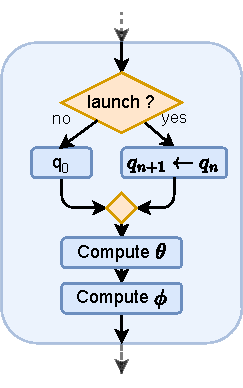
\includegraphics[width=0.9\textwidth]{figures/elec/calcul_attitude.drawio.pdf}
		\caption{Calcul d'attitude}
	\end{figure}
\end{minipage}
\hfill

\newpage

\subsubsubsection{Comparaison avec les valeurs attendues}

Les valeurs d'attitude étant calculées, le séquenceur doit s'en servir afin de déterminer si l'allumage du propulseur du second
étage est autorisé.

\hspace*{-\parindent}%
\begin{minipage}{0.35\textwidth}
	\begin{figure}[H]
		\centering
		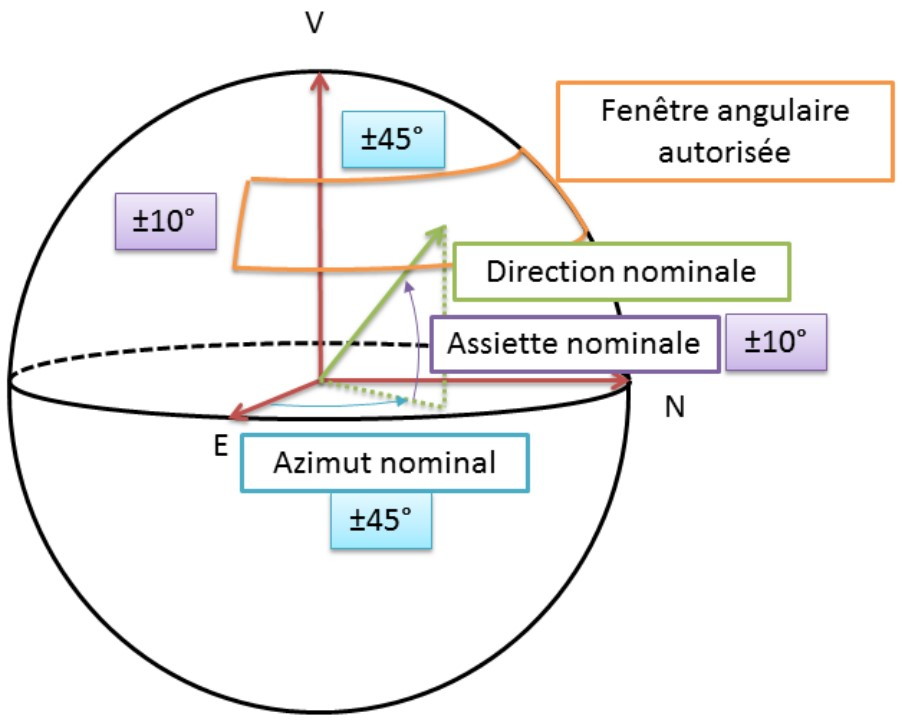
\includegraphics[width=\textwidth]{figures/elec/fenetre_attitude.jpg}
		\caption{Fenêtre d'attitude autorisée pour l'allumage du propulseur du second étage.}
	\end{figure}
\end{minipage}
\hfill
\begin{minipage}{0.6\textwidth}
	Les conditions d'allumage sont les suivantes :
	\begin{itemize}
		\item l'angle d'élévation $\theta_n$ doit se trouver dans un intervalle de tolérence de $\pm10°$ autour de l'angle
		d'élévation nominal $\theta_{nom,n}$ ;
		\item l'angle d'azimut $\phi_n$ doit se trouver dans un intervalle de tolérence de $\pm45°$ autour de l'angle
		d'azimut nominal $\phi_{nom,n}$.
	\end{itemize}
	Ces angles nominaux représentent ceux que la fusée doit théoriquement atteindre à l'instant $t_n$ lors d'un vol stable sans
	vent et sans perturbation. L'angle $\phi_{nom,n}$ est déterminé par la direction choisi par les équipes du \acrshort{CNES}
	lors de l'orientation de la rampe de lancement. L'angle $\theta_{nom,n}$ est lui déterminé via la simulation de vol donnée
	par le \gls{Stabtraj}.
\end{minipage}

\vspace{0.4cm}

A l'aide d'Excel, l'évolution théorique de l'angle d'élévation $\theta_{nom,n}$ a été modélisé en fonction du temps par une
équation polynomiale du 3ème degré. 

\begin{figure}[H]
	\centering
	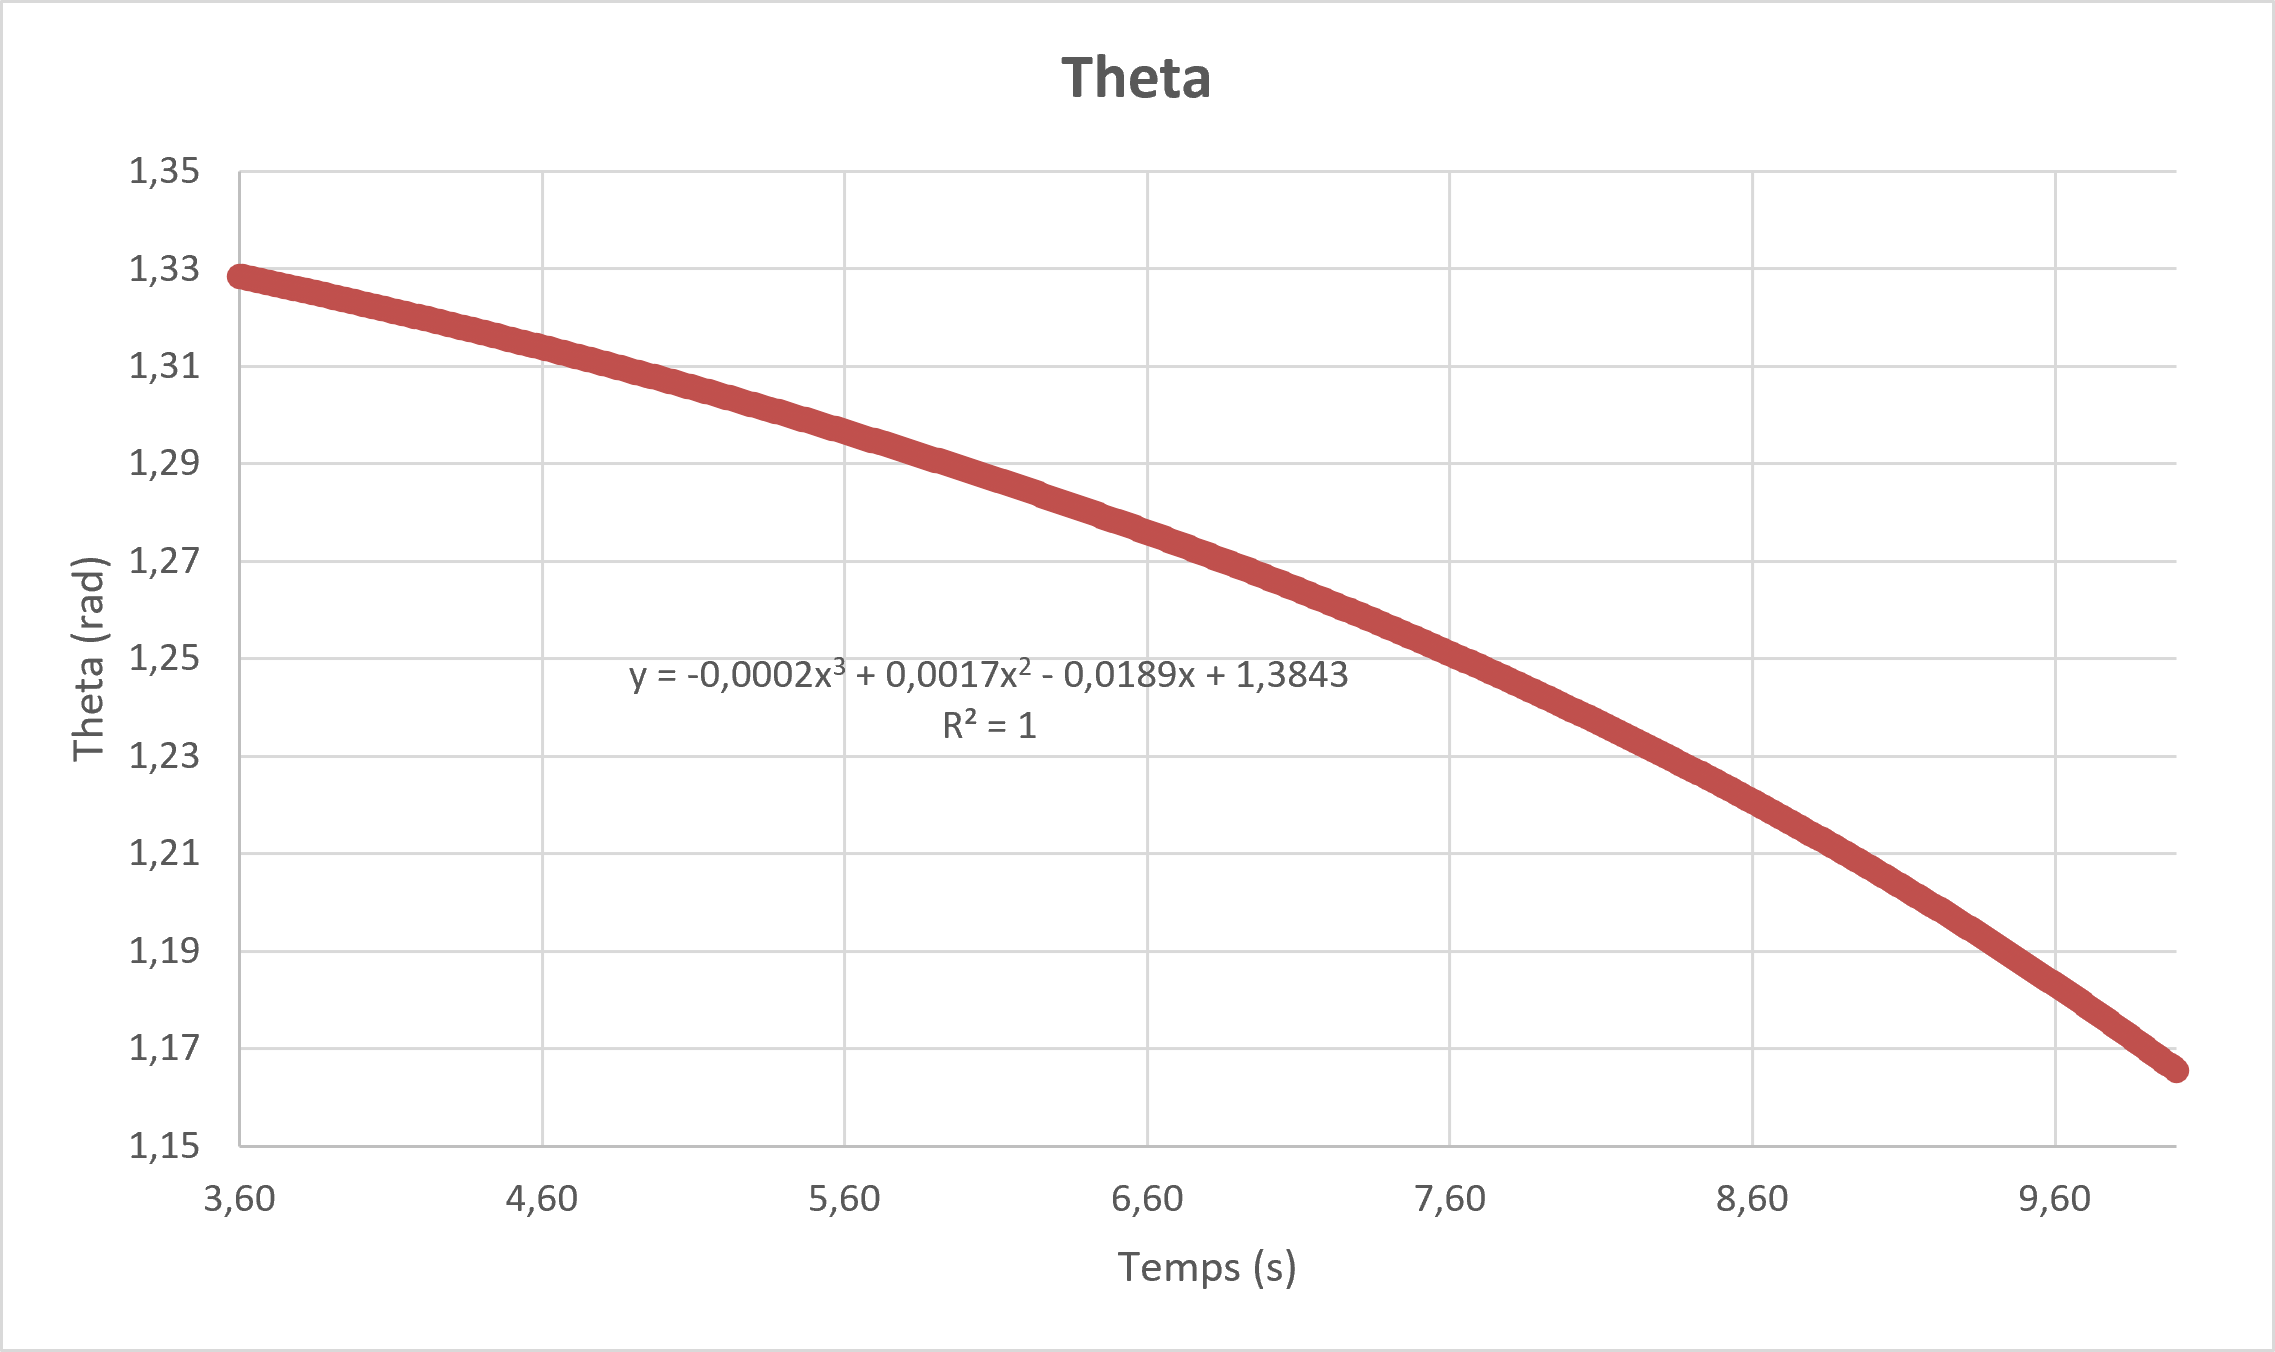
\includegraphics[width=0.8\textwidth]{figures/elec/theta_excel.png}
	\caption{Fenêtre d'attitude autorisée pour l'allumage du propulseur du second étage.}
\end{figure}

% y = -0,0002x3 + 0,0017x2 - 0,0189x + 1,3843 ; R² = 1

La méthode des moindre carrés a été utilisée sur une portion du vol allant de \SI{3.6}{\second} à \SI{10.0}{\second}. Sur
cette portion de vol, l'évolution de l'angle d'élévation est modélisé par l'équation polynomiale suivante :
\begin{equation}
	\theta_{nom,n} = -0.0002 t_n^3 + 0.0017 t_n^2 - 0.0189 t_n + 1.3843
\end{equation}
Le coefficient de détermination $R^2$ est très proche de 1, ce qui signifie que l'équation polynomiale du 3ème degré est une
bonne approximation de l'évolution de l'angle théorique.\\

A chaque itération, la condition d'allumage est alors :

\begin{equation}
	\begin{cases}
		\left\|\Delta \theta_n\right\| = \left\|\theta_{nom,n} - \theta_n \right\| \leq 10\degres \\
		\left\|\Delta \phi_n \right\| = \left\|\phi_{nom,n} - \phi_n \right\| \leq 45\degres
	\end{cases}
\end{equation}

\newpage

\subsubsection{Bibliothèques logicielles du séquenceur}

Cette section présente quelques bibliothèques logicielles développées pour le projet et utilisées par le séquenceur. Elles sont
détaillées ici pour leur intérêt pédagogique et pour la compréhension du niveau d'abstraction atteint par le programme du
séquenceur.

\subsubsubsection{Contrôle des actionneurs}
\label{subsubsubsec:seq_actionneurs}

Les organes mécaniques de la fusée (aérofreins, trappes de parachute, système de séparation) sont tous mus par des servomoteurs
Feetech STS3215. Leur commande repose sur deux bibliothèques logicielles :
\begin{itemize}
    \item le pilote \texttt{STS}, qui implémente le protocole série du servomoteur ;
    \item l'utilitaire \texttt{actuator}, qui créer une couche d'abstraction du système mécanique dans lequel il se place.
\end{itemize}
Ce dernier permet de gérer les actionneurs de manière plus abstraite, en permettant de désigner une liste de positions pour
chaque système, de passer d'une position à une autre simplement et de pouvoir effectuer une calibration en trouvant les points de
référence de chaque système mécanique. La figure \ref{fig:sts_actuator} représente l'articulation de ces deux couches.

\begin{figure}[H]
    \centering
    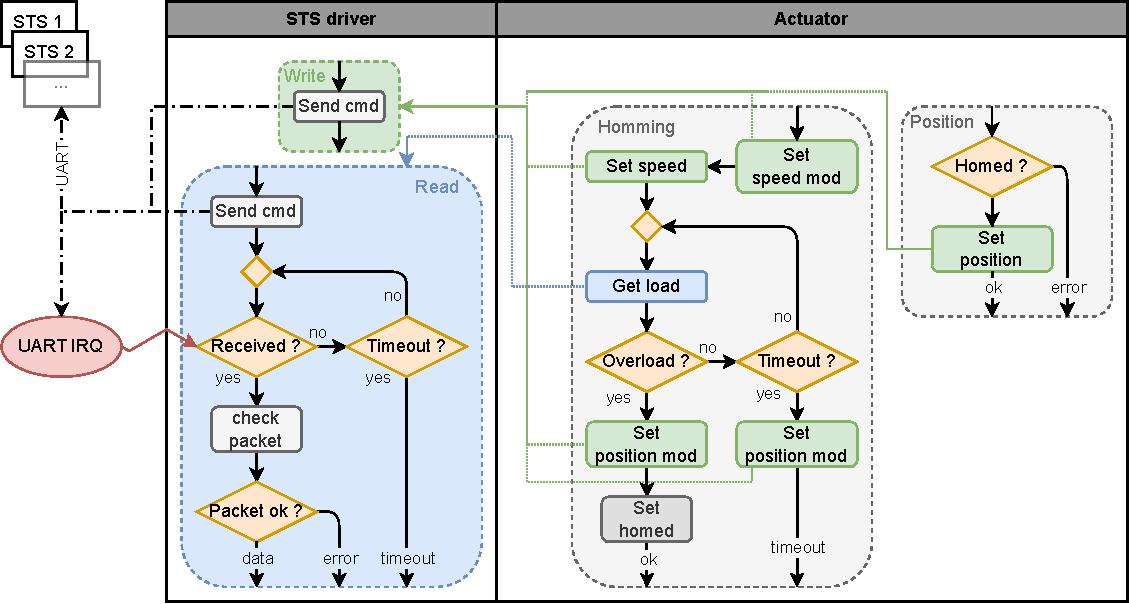
\includegraphics[width=0.95\textwidth]{figures/elec/STS_actuator.drawio.pdf}
    \caption{Articulation du pilote \texttt{STS} et de l'utilitaire \texttt{actuator}}
    \label{fig:sts_actuator}
\end{figure}

\vspace{-0.4cm}

\subparagraph*{Un bus série partagé et protocole de communication} Comme dit précédemment en partie \ref{subsec:elec_servomoteur},
les servomoteurs utilisés dans le projet communiquent sur un bus série partagé \texttt{UART Half-Duplex}.

\vspace{0.1cm}

\hspace*{-\parindent}%
\begin{minipage}{0.45\textwidth}
Le protocole de communication est propriétaire et documenté par le fabricant. Les servomoteurs sont des composants esclaves qui
agissent et répondent aux commandes envoyées par le microcontrôleur maître. Le protocole se découpe en deux types de trames :
\begin{itemize}
	\item les trames d'instruction, qui contiennent les ordres envoyés par le microcontrôleur maître vers le servomoteur esclave ;
	\item les trames de réponse, qui contiennent les réponses du servomoteur esclave vers le microcontrôleur maître.
\end{itemize}
\end{minipage}
\hfill
\begin{minipage}{0.5\textwidth}
	\begin{table}[H]
		\centering
		\begin{tabular}{l l | l l}
			\hline
			\multicolumn{2}{l|}{\textbf{Trames d'instruction}} & \multicolumn{2}{l}{\textbf{Trames de réponse}} \\
			\hline
			Taille	& Nom			& Taille	& Nom			\\
			2		& Préambule		& 2			& Préambule		\\
			1		& Identifiant	& 1			& Identifiant	\\
			1		& Longueur		& 1			& Longueur		\\
			1		& Instruction	& 1			& Code d'erreur	\\
			N		& Paramètres	& N			& Paramètres	\\
			1		& checksum		& 1			& checksum		\\
			\hline
		\end{tabular}
		\caption{Types de trames dans le protocole série du servomoteur Feetech STS3215}
		\label{tab:sts_trames}
	\end{table}
\end{minipage}

\vspace{0.1cm}

Le tableau \ref{tab:sts_trames} résume les différents types de trames et leur rôle dans le protocole.

\newpage

\subparagraph*{Read / Write} La figure distingue deux chemins d'exécution dans le pilote. \textit{Write} Consiste à l'envoie d'une
trame d'instruction vers le servmoteur sans attente de réponse. Toute opération sur un servomoteur se rapporte à l'écriture d'une
valeur dans un registre de celui-ci. \textit{Read} cependant nécessite deux actions : l'envoi d'une trame d'instruction vers le
servomoteur, puis la lecture de la trame de réponse. Lorsque le pilote est sollicité pour lire un registre, il envoie la trame
d'instruction correspondante, puis attend la réponse du servomoteur via une interruption matérielle sur le bus série concerné. Le
pilote vérifie ensuite la validité de la trame reçue et en extrait la valeur du registre demandé. Si la trame n'est pas valide, le
pilote signale une erreur. Egalement, si aucune réponse n'est reçue dans un délai fixé, le pilote signale un timeout.\\

L'aspect partagé du bus série est géré par le pilote d'une manière très simplifié mais robuste, efficace et suffisante pour le
projet. Le logiciel du séquenceur ne s'adresse qu'à un servomoteur à la fois. Puisque les servomoteurs agissent comme des
esclaves, il n'y a pas de risque de collision sur le bus série. Lors d'une opération de lecture, le pilote attend la réponse
provenant nécessairement du dernier servomoteur solicitée. Le champ d'identifiant dans la trame de réponse permet de vérifier que
la réponse provient bien du bon servomoteur.\\

L'abstraction de ce protocole et la gestion des mécanismes de \textit{Read / Write} sont encapsulés dans le pilote \texttt{STS}.

\vspace{0.8cm}

% \hspace*{-\parindent}%
\begin{minipage}{0.32\textwidth}
\subparagraph*{L'abstraction d'un actionneur} L'utilitaire \texttt{actuator}  associe à chaque servomoteur une configuration
décrivant l'organe qu'il motorise, et conserve l'état de cet organe :
	
La configuration énumère les positions utiles d'un actionneur, exprimées en degrés, et désigne parmi elles celle qui correspond à
sa butée mécanique. Le reste du programme n'a donc jamais à manipuler d'angle : il demande une position par son indice, et la
conversion reste interne à la bibliothèque.
\end{minipage}
\hfill
\begin{minipage}{0.50\textwidth}
\begin{lstlisting}[language=C, frame=tb, basicstyle=\small]
// .../utils/actuator.h

typedef struct {
    float   homing_speed_rpm;
    uint8_t homing_calibration_idx;
    float   positions_deg[256];
    uint8_t num_positions;
} Actuator_Config_t;

typedef struct Actuator_t {
    STS_Servo_t       *servo;
    Actuator_Config_t  config;
    bool               is_homed;
    uint8_t            current_position;
    ...
} Actuator_t;
\end{lstlisting}
\end{minipage}
\hfill
\hfill


\subparagraph*{Mise en référence} Les positions n'ont de sens qu'une fois le repère interne du servomoteur mis en correspondance
avec le repère mécanique du système mécanique qu'il contrôle. Les servomoteurs utilisés dans le projet disposant d'un suivi du
couple exercé, les points de référence les plus simples à détecter sont les butées mécaniques de chaque actionneur. La mise en
référence consiste donc à déplacer le servomoteur jusqu'à ce qu'il atteigne sa butée, puis à marquer cette position comme repère.\\

La procédure, représentée sur la figure \ref{fig:sts_actuator}, bascule le servomoteur en commande de vitesse, le déplace à
vitesse réduite en direction de la butée, puis surveille sa charge jusqu'à détecter la surcharge caractéristique du blocage. Le
servomoteur est alors calibré, repassé en commande de position, et l'actionneur est marqué comme référencé.\\

Cette opération dure plusieurs secondes et ne peut donc pas immobiliser la boucle. Non représenté dans la figure par soucis de
simplicité, elle est découpée en étapes internes, chaque appel faisant progresser la procédure d'un pas avant de rendre la main
(le même motif que celui employé pour les fonctions sol en section \ref{par:seq_ground_funcs}). Si la procédure de mise en
référence dépasse un délai fixé, elle est abandonnée et l'actionneur n'est pas marqué comme référencé. Toute commande de position
ultérieure sera alors refusée, conformément à la vérification effectuée en début de chemin de commande. Cela permet d'éviter
d'ordonner un mouvement à un actionneur qui n'aurait pas été correctement calibré, ce qui pourrait conduire à une collision
mécanique et potentiellement à un endommagement de la fusée. Les systèmes mécaniques étant couteux en temps de travail et en
argent, il est préférable de prévenir toute erreur de manipulation.

\newpage

\subsubsubsection{Gestion des événements lumineux}
\label{subsubsubsec:seq_leds}

\paragraph*{Motivation} La LED est l'unique canal de communication en temps réel vers l'opérateur au sol. Le programme du
séquenceur a cependant une exécution non linéaire : à un instant donné, plusieurs conditions peuvent être vraies ou en attente
simultanément, plutôt qu'un unique état à la fois. L'opérateur doit donc pouvoir déterminer, par la seule observation de la LED,
ce qu'il se passe : si le séquenceur attend une action, laquelle, et si une condition est remplie ou non, ycompris lorsque
plusieurs de ces informations sont pertinentes en même temps. Une couleur fixe par état ne suffit ni à distinguer un nombre
suffisant de situations, ni à signaler qu'une condition est en cours d'évaluation plutôt qu'acquise. Le choix retenu est de
représenter chaque condition par un motif dans le temps plutôt que par une couleur statique, ce qui nécessite une abstraction
manipulant le temps : c'est le rôle de la bibliothèque \texttt{waveform}, qui permet de définir un nombre arbitraire de motifs
distincts. Plusieurs motifs pouvant être actifs simultanément, il faut ensuite un mécanisme qui les fasse cohabiter sans
qu'aucune partie du programme n'ait à connaître ce qui est affiché par ailleurs : c'est le rôle de l'ordonnanceur
\texttt{led\_scheduler}.

\paragraph{Modèle temporel} Un motif lumineux est représenté par une fonction du temps, indépendante de la couleur ou de
l'intensité qu'il portera une fois affiché. Deux domaines sont distingués selon la nature de la grandeur représentée : un motif
d'intensité est une fonction $f_{1D} : [0,1] \to [0,1]$, tandis qu'un motif de couleur est une fonction $f_{3D} : [0,1] \to [0,1]^3$
dont les trois composantes correspondent aux canaux rouge, vert et bleu de la LED.\\

La figure~\ref{fig:waveform_fa} illustre un motif d'intensité $f_a(t)$ construit à titre d'exemple : une bosse sinusoïdale
suivie de deux portes de largeurs différentes, dont la somme est bornée à $[0,1]$.

% $$ f_a(t) = \max(0, \min(1, \text{bosse}(t, 0, 0.4) + \text{porte}(t, 0.35, 0.6) + \text{porte}(t, 0.75, 0.8))) $$
$$ f_a(t) = \text{clap}\left(0, 1, \left[0.5 - 0.5 \cos{\left(2\pi\frac{t - 0.2}{0.4}\right)}\right]\prod\left(\frac{t-0.2}{0.4}\right) + \bigwedge\left(\frac{t-0.4}{0.2}\right)+ \prod\left(\frac{t-0.8}{0.1}\right)\right)$$ % )) $$

\noindent où $\text{clap}(a, b, x) = \max(a, \min(b, x))$ est la fonction de limitation à l'intervalle
$[a,b]$, $\prod(x)$ est la fonction porte définie par $\prod(x) = \left\{1 \text{ si } -\frac{1}{2} \leq x < \frac{1}{2}, 0 \text{ sinon}\right\}$
et $\bigwedge(x)$ est la fonction triangle définie par $\bigwedge(x) = \left\{1 - |2x| \text{ si } -\frac{1}{2} \leq x < \frac{1}{2}, 0 \text{ sinon}\right\}$.\\

\pgfplotsset{compat=1.18}

% ---- Paramètres génériques (à modifier ici uniquement) ----
\pgfmathsetmacro{\SinStart}{0}
\pgfmathsetmacro{\SinEnd}{0.4}
\pgfmathsetmacro{\GateOneStart}{0.3}
\pgfmathsetmacro{\GateOneEnd}{0.5}
\pgfmathsetmacro{\GateTwoStart}{0.75}
\pgfmathsetmacro{\GateTwoEnd}{0.85}
\pgfmathsetmacro{\Dephasage}{1/50}

% ---- Formes de base ----
\pgfmathdeclarefunction{gate}{3}{%
  \pgfmathparse{ifthenelse((#1 >= #2) && (#1 < #3), 1, 0)}%
}
\pgfmathdeclarefunction{bosse}{3}{%
  \pgfmathparse{ifthenelse((#1 >= #2) && (#1 < #3), 0.5 - 0.5*cos(360*(#1-#2)/(#3-#2)), 0)}%
}
\pgfmathdeclarefunction{clap}{3}{%
  \pgfmathparse{min(#1, max(#2, #3))}%
}
\pgfmathdeclarefunction{triangle}{3}{%
  \pgfmathparse{ifthenelse((#1 >= #2) && (#1 < #3), 1 - abs(2*(#1-#2)/(#3-#2)-1), 0)}%
}

% ---- f_a(t) : composition bornée ----
\pgfmathdeclarefunction{fa}{1}{%
  \pgfmathparse{min(1, max(0, %
    bosse(#1,\SinStart,\SinEnd) + triangle(#1,\GateOneStart,\GateOneEnd) + gate(#1,\GateTwoStart,\GateTwoEnd) %
  ))}%
}

% ---- f_b(t) : f_a déphasée sur les 3 voies ----
\pgfmathdeclarefunction{wrap}{1}{\pgfmathparse{#1 - floor(#1)}}
\pgfmathdeclarefunction{fbR}{1}{\pgfmathparse{fa(wrap(#1))}}
\pgfmathdeclarefunction{fbG}{1}{\pgfmathparse{fa(wrap(#1-\Dephasage))}}
\pgfmathdeclarefunction{fbB}{1}{\pgfmathparse{fa(wrap(#1-2*\Dephasage))}}

\vspace{-0.4cm}

\begin{figure}[H]
\centering
\begin{tikzpicture}
\begin{axis}[
    width=0.9\linewidth, height=4.5cm,
    xlabel={$t$}, ylabel={$f_a(t)$},
    xmin=0, xmax=1, ymin=-0.05, ymax=1.15,
    xtick={0,0.2,0.4,0.6,0.8,1}, ytick={0,0.5,1},
    axis lines=left,
    domain=0:1, samples=200,
    legend pos=outer north east,
]
\addplot[thick, black] {fa(x)}; \addlegendentry{$I$}
\end{axis}
\end{tikzpicture}
\caption{Motif $f_a(t)$ : bosse sinusoïdale suivie de deux portes de largeurs différentes.}
\label{fig:waveform_fa}
\end{figure}

\vspace{-0.4cm}

La figure~\ref{fig:waveform_fb} illustre un motif de couleur $f_b(t)$ construit à partir de $f_a$, en appliquant le même motif à
chacun des trois canaux avec un déphasage entre eux.

\begin{figure}[H]
\centering
\begin{tikzpicture}
\begin{axis}[
    width=0.9\linewidth, height=4.5cm,
    xlabel={$t$}, ylabel={$f_b(t)$},
    xmin=0, xmax=1, ymin=-0.05, ymax=1.15,
    xtick={0,0.2,0.4,0.6,0.8,1}, ytick={0,0.5,1},
    axis lines=left,
    domain=0:1, samples=200,
    legend pos=outer north east,
]
\addplot[thick, red] {fbR(x)}; \addlegendentry{$R$}
\addplot[thick, green!60!black] {fbG(x)}; \addlegendentry{$G$}
\addplot[thick, blue] {fbB(x)}; \addlegendentry{$B$}
\end{axis}
\end{tikzpicture}
\caption{Motif $f_b(t)$ : même motif que $f_a$, déphasé d'un décalage $\Delta = 1/50$ entre chaque voie colorimétrique.}
\label{fig:waveform_fb}
\end{figure}

\newpage

\paragraph*{Structure générique} Pour être manipulé de façon uniforme (combiné avec d'autres motifs), un motif doit exposer une
même interface, quelle que soit sa nature ou sa complexité. Une fonction associée à un motif d'intensité ou
\textit{wave\_func\_scalar\_t} ($f_{1D}$) et une fonction associée à un motif de couleur ou \textit{wave\_func\_space\_t}
($f_{3D}$) ne prennent donc, l'une comme l'autre, que deux arguments : la phase $t$, et un pointeur de contexte non typé
(\texttt{const void *}).\\

\begin{lstlisting}[language=C, frame=tb, basicstyle=\small]
// t in [0, 1] ; returns intensity in [0, 1]
typedef float (*wave_func_scalar_t)(float t, const void *ctx);

// t in [0, 1] ; returns  color in [0, 1]^3
typedef float3_t (*wave_func_space_t)(float t, const void *ctx);
\end{lstlisting}

Ce pointeur de contexte permet à chaque fonction de recevoir les paramètres qui lui sont propres (les bornes d'une porte, le
coefficient de décroissance d'une impulsion, ou les motifs et facteurs à combiner) sans que cela n'altère la signature commune.
Chaque fonction se charge elle-même de convertir ce pointeur vers le type de structure qu'elle attend. C'est ce mécanisme qui
permet de traiter indifféremment un motif élémentaire ou une composition de plusieurs motifs : les deux exposent la même
interface, seul le contenu du contexte diffère.

\paragraph*{Formes de base et opérateurs de composition} La bibliothèque fournit un petit nombre de motifs de base, prêtes à
l'emploi (tableau~\ref{tab:formes_base}), ainsi que des opérateurs arithmétiques permettant de les combiner entre elles ou avec
des constantes (tableau~\ref{tab:operateurs}). Un opérateur de composition expose la même interface qu'une forme de base : son
contexte contient simplement les motifs (fonction et pointeur de contexte) sur lesquels il opère, ce qui lui permet d'être à
son tour combiné avec d'autres motifs, y compris d'autres compositions.\\


\begin{table}[h]
\centering
\begin{tabular}{p{6cm} l p{6.2cm} }
\hline
\textbf{Description} & \textbf{Attribut} & \textbf{Description de l'attribut} \\
\hline

\multicolumn{3}{l}{\texttt{gate}} \\
\hline
\multirow{2}{6cm}{Intensité de 1 sur l'intervalle actif, 0 en dehors} &
\texttt{start} & Borne inférieure de l'intervalle actif \\
\cline{2-3}
 & \texttt{end} & Borne supérieure de l'intervalle actif \\
\hline

\multicolumn{3}{l}{\texttt{ramp}} \\
\hline
\multirow{2}{6cm}{Rampe linéaire croissante sur l'intervalle actif} &
\texttt{start} & Borne inférieure de l'intervalle actif \\
\cline{2-3}
 & \texttt{end} & Borne supérieure de l'intervalle actif \\
\hline

\multicolumn{3}{l}{\texttt{triangle}} \\
\hline
\multirow{2}{6cm}{Montée puis descente linéaires sur l'intervalle actif} &
\texttt{start} & Borne inférieure de l'intervalle actif \\
\cline{2-3}
 & \texttt{end} & Borne supérieure de l'intervalle actif \\
\hline

\multicolumn{3}{l}{\texttt{sine}} \\
\hline
\multirow{2}{6cm}{Bosse sinusoïdale (montée puis descente) sur l'intervalle actif} &
\texttt{start} & Borne inférieure de l'intervalle actif \\
\cline{2-3}
 & \texttt{end} & Borne supérieure de l'intervalle actif \\
\hline

\multicolumn{3}{l}{\texttt{impulse}} \\
\hline
\multirow{3}{6cm}{Décroissance exponentielle sur l'intervalle actif} &
\texttt{start} & Borne inférieure de l'intervalle actif \\
\cline{2-3}
 & \texttt{end} & Borne supérieure de l'intervalle actif \\
\cline{2-3}
 & \texttt{k} & Coefficient de décroissance exponentielle \\
\hline

\end{tabular}
\caption{Formes de base de la bibliothèque \texttt{waveform}}
\label{tab:formes_base}
\end{table}


\begin{table}[H]
\centering
\begin{tabular}{p{5.5cm} l p{5.5cm}}
\hline
\textbf{Description} & \textbf{Attribut} & \textbf{Description de l'attribut} \\
\hline

\multicolumn{3}{l}{\texttt{scale\_add\_const}} \\
\hline
\multirow{3}{5cm}{Ajoute une constante à une fonction scalaire} &
\texttt{wave\_function\_add} & Fonction \\
\cline{2-3}
 & \texttt{ctx\_add} & Contexte de la fonction \\
\cline{2-3}
 & \texttt{offset} & Constante ajoutée \\
\hline

\multicolumn{3}{l}{\texttt{scale\_add}} \\
\hline
\multirow{3}{5cm}{Additionne deux fonctions scalaires} &
\texttt{wave\_function\_add\_1} & 1er fonction \\
\cline{2-3}
 & \texttt{ctx\_add\_1} & Contexte de la 1ere fonction \\
\cline{2-3}
 & \texttt{wave\_function\_add\_2} & 2e fonction \\
\cline{2-3}
 & \texttt{ctx\_add\_2} & Contexte de la 2e fonction \\
\hline

\multicolumn{3}{l}{\texttt{scale\_mult\_const}} \\
\hline
\multirow{3}{5cm}{Multiplie une fonction scalaire par une constante} &
\texttt{wave\_function\_mult} & Fonction \\
\cline{2-3}
 & \texttt{ctx\_mult} & Contexte de la fonction \\
\cline{2-3}
 & \texttt{factor} & Constante multiplicative \\
\hline

\multicolumn{3}{l}{\texttt{scale\_mult}} \\
\hline
\multirow{3}{5cm}{Multiplie deux fonctions scalaires} &
\texttt{wave\_function\_mult\_1} & 1er fonction \\
\cline{2-3}
 & \texttt{ctx\_mult\_1} & Contexte de la 1ere fonction \\
\cline{2-3}
 & \texttt{wave\_function\_mult\_2} & 2e fonction \\
\cline{2-3}
 & \texttt{ctx\_mult\_2} & Contexte de la 2e fonction \\
\hline

\multicolumn{3}{l}{\texttt{space\_add\_const}} \\
\hline
\multirow{3}{5cm}{Ajoute une couleur constante à une fonction spatiale} &
\texttt{wave\_function\_add} & Fonction  \\
\cline{2-3}
 & \texttt{ctx\_add} & Contexte de la fonction \\
\cline{2-3}
 & \texttt{offset} & Couleur ajoutée \\
\hline

\multicolumn{3}{l}{\texttt{space\_add}} \\
\hline
\multirow{4}{5cm}{Additionne deux fonctions spatiales} &
\texttt{wave\_function\_add\_1} & 1er fonction \\
\cline{2-3}
 & \texttt{ctx\_add\_1} & Contexte de la 1ere fonction \\
\cline{2-3}
 & \texttt{wave\_function\_add\_2} & 2e fonction \\
\cline{2-3}
 & \texttt{ctx\_add\_2} & Contexte de la 2e fonction \\
\hline

\multicolumn{3}{l}{\texttt{space\_mult\_const}} \\
\hline
\multirow{3}{5cm}{Multiplie une fonction scalaire par une couleur constante} &
\texttt{wave\_function\_mult} & Fonction scalaire \\
\cline{2-3}
 & \texttt{ctx\_mult} & Contexte de la fonction scalaire \\
\cline{2-3}
 & \texttt{factor} & Couleur de référence \\
\hline

\end{tabular}
\caption{Opérateurs de composition de la bibliothèque \texttt{waveform}}
\label{tab:operateurs}
\end{table}

Parmi ces opérateurs, un cas particulier assure la transition entre les deux domaines introduits précédemment :
\texttt{space\_mult\_const} met à l'échelle une couleur constante par un motif d'intensité, convertissant ainsi un motif
d'intensité en motif de couleur.

\paragraph*{Persistance et temporalité} Une forme de base ou une composition, telle que décrite précédemment, n'est qu'une
fonction pure de la phase : elle ne conserve aucun état d'un appel à l'autre. Pour être effectivement jouée, elle est
enveloppée dans une structure qui lui associe une temporalité propre : une durée $T$, un indicateur de périodicité, ainsi qu'une
horloge interne démarrée au premier instant où le motif est effectivement évalué. Un motif non périodique devient inactif dès
que sa durée s'est écoulée une fois. Un motif périodique reprend au contraire indéfiniment à $t=0$ à l'issue de chaque période.\\

\noindent La composition de cette structure avec la fonction forme l'entité complète d'un motif appelé \texttt{waveform}.

\newpage

\paragraph{Exemple de composition} Le code ci-dessous illustre la construction d'un motif de couleur à partir des seules formes
de base et opérateurs de composition présentés précédemment, sans qu'aucune fonction supplémentaire ne soit écrite. Le motif
obtenu additionne deux contributions :
\begin{itemize}
	\item une décroissance exponentielle combinée à une porte, toutes deux mises à l'échelle d'une même teinte
	\item une bosse sinusoïdale, mise à l'échelle d'une seconde teinte.
\end{itemize}
Chaque opérateur ne fait que porter, dans son contexte, les motifs et les paramètres sur lesquels il opère. La structure du
code reflète directement l'arbre de composition du motif.
\begin{lstlisting}[language=C, frame=tb, basicstyle=\small]
const waveform_space_add_t wfm_exemple_ctx = {
    .wave_function_add_1 = waveform_space_mult_const,
    .ctx_add_1 = &(const waveform_space_mult_const_t) {
        .wave_function_mult = waveform_scale_add,
        .ctx_mult = &(const waveform_scale_add_t) {
            .wave_function_add_1 = waveform_impulse,
            .ctx_add_1 = &(const waveform_impulse_t) {
                .start = 0.2f,
                .end = 0.4f,
                .k = 5.0f
            },
            .wave_function_add_2 = waveform_gate,
            .ctx_add_2 = &(const waveform_gate_t) {
                .start = 0.8f,
                .end = 0.9f
            },
        },
        .factor = (float3_t){ .x = 0.2f, .y = 0.7f, .z = 0.8f }
    },
    .wave_function_add_2 = waveform_space_mult_const,
    .ctx_add_2 = &(const waveform_space_mult_const_t) {
        .wave_function_mult = waveform_sine,
        .ctx_mult = &(const waveform_sine_t) {
            .start = 0.3f,
            .end = 0.7f,
        },
        .factor = (float3_t){ .x = 1.0f, .y = 0.8f, .z = 0.0f }
    }
};
\end{lstlisting}

\vfill

\noindent La figure~\ref{fig:waveform_exemple} représente l'exécution de ce motif sur les trois canaux de couleur en fonction de
la phase $t$.

% Nouvelles déclarations : gate et bosse sont déjà définies plus haut (figures f_a/f_b),
% ne pas les redéclarer sous peine d'erreur de compilation.
\pgfmathdeclarefunction{impulse}{4}{%
  \pgfmathparse{ifthenelse((#1 >= #2) && (#1 < #3), exp(-#4*(#1-#2)/(#3-#2)), 0)}%
}
\pgfmathdeclarefunction{branchA}{1}{%
  \pgfmathparse{impulse(#1,0.2,0.4,5) + gate(#1,0.8,0.9)}%
}
\pgfmathdeclarefunction{branchB}{1}{%
  \pgfmathparse{bosse(#1,0.3,0.7)}%
}
\pgfmathdeclarefunction{ExR}{1}{\pgfmathparse{0.2*branchA(#1) + 1.0*branchB(#1)}}
\pgfmathdeclarefunction{ExG}{1}{\pgfmathparse{0.7*branchA(#1) + 0.8*branchB(#1)}}
\pgfmathdeclarefunction{ExB}{1}{\pgfmathparse{0.8*branchA(#1) + 0.0*branchB(#1)}}

\begin{figure}[h]
	\centering
	\begin{tikzpicture}
		\begin{axis}[
			width=0.9\linewidth, height=5cm,
			xlabel={$t$}, ylabel={intensité},
			xmin=0, xmax=1, ymin=-0.05, ymax=1.15,
			xtick={0,0.2,0.4,0.6,0.8,1}, ytick={0,0.5,1},
			axis lines=left,
			domain=0:1, samples=200,
			legend pos=outer north east,
		]
			\addplot[thick, red] {ExR(x)}; \addlegendentry{$R$}
			\addplot[thick, green!60!black] {ExG(x)}; \addlegendentry{$G$}
			\addplot[thick, blue] {ExB(x)}; \addlegendentry{$B$}
		\end{axis}
	\end{tikzpicture}
	\caption{Exécution du motif sur les trois canaux de couleur.}
	\label{fig:waveform_exemple}
\end{figure}

\vfill\vfill

\newpage

Une fois défini, ce motif est instancié dans la structure introduite précédemment, avec une durée de 5 secondes et un
fonctionnement périodique. Il peut ensuite être joué par dans une boucle infinie. Le pointeur \texttt{wfm} représente le motif
à jouer, et est passé à la fonction \texttt{Waveform\_Play\_Space} à chaque itération. Cette fonction ne fait qu'évaluer le
motif à l'instant courant, et renvoie la couleur correspondante. Ce résultat est ensuite transmis à la LED.

\begin{lstlisting}[language=C, frame=tb, basicstyle=\small]
waveform_space_t waveform_exemple;
Waveform_Init_Space(
	&wfm_exemple,
	waveform_space_add,
	&wfm_exemple_ctx,
	5000,
	true
);

waveform_space_t *wfm = &wfm_exemple;
while (1) {
    float3_t result = Waveform_Play_Space(
		wfm,
		HAL_GetTick()
	);
    LED_RGB_SetColor(&led_rgb, result);
}
\end{lstlisting}

\newpage

\paragraph*{LED\_SCHEDULER} Là où la bibliothèque \texttt{waveform} décrit un motif lumineux, l'ordonnanceur
\texttt{led\_scheduler} détermine, à chaque itération de boucle, lesquels des motifs actifs sont visibles et comment ils se
combinent en une unique couleur. L'unité manipulée par l'ordonnanceur est l'événement lumineux : un motif de couleur, associé
aux règles qui régissent sa cohabitation avec les autres événements. L'ensemble de l'interface exposée à l'utilisateur est
donné par le code ci-dessous.

\begin{lstlisting}[language=C, frame=tb, basicstyle=\small]
#define LED_SCHED_MAX_EVENTS 8	// Aribitraire. Peut etre augmente si besoin

typedef int32_t led_evt_handle_t;
#define LED_SCHED_HANDLE_INVALID ((led_evt_handle_t)-1)

typedef enum {
    LED_SCHED_NO_FORCE,
    LED_SCHED_SOFT_FORCE,
    LED_SCHED_HARD_FORCE,
} led_evt_force_t;

void             LedSched_Init(void);
led_evt_handle_t LedSched_Add(waveform_space_t *waveform, uint8_t priority,
                              bool transparent, uint32_t pause_timeout_ms,
                              led_evt_force_t force);
void             LedSched_Remove(led_evt_handle_t evt);
void             LedSched_Clear(void);
bool             LedSched_IsHandleValid(led_evt_handle_t evt);
float3_t         LedSched_Process(uint32_t now_ms);
\end{lstlisting}

L'ajout d'un événement est réalisé par \texttt{LedSched\_Add}, dont les cinq paramètres, détaillés dans le
tableau~\ref{tab:led_sched_add}, suffisent à définir l'intégralité de son comportement. La fonction renvoie un identifiant de
l'événement créé, ou la valeur \texttt{LED\_SCHED\_HANDLE\_INVALID} si l'ajout a échoué. La capacité de l'ordonnanceur est
fixée à la compilation par \texttt{LED\_SCHED\_MAX\_EVENTS} : les événements sont stockés dans une \og pool \fg{} (réserve)
statique, sans allocation dynamique.

\begin{table}[H]
\centering
\begin{tabular}{|l|>{\raggedright\arraybackslash}p{3.5cm}|l|>{\raggedright\arraybackslash}p{5.75cm}|}
\hline
\textbf{Paramètre} & \textbf{Description} & \textbf{Valeur} & \textbf{Effet} \\
\hline
\texttt{waveform} & Motif de couleur joué par l'événement & -- & Le motif est redémarré à l'ajout \\
\hline
\texttt{priority} & Niveau de visibilité de l'événement & $0$ à $255$ & Une valeur plus élevée correspond à un événement plus prioritaire \\
\hline
\multirow{2}{*}{\texttt{transparent}} & \multirow{2}{3cm}{Mode de cohabitation avec les autres événements} & \texttt{false} & Opaque : masque les événements de priorité inférieure \\
\cline{3-4}
 & & \texttt{true} & Transparent : la couleur s'additionne à celle des autres événements visibles \\
\hline
\multirow{3}{*}{\texttt{timeout\_ms}} & \multirow{3}{3cm}{Comportement de l'événement lorsqu'il est masqué} & $0$ & Jamais mis en pause : le motif continue de s'écouler sans être affiché \\
\cline{3-4}
 & & Autre valeur $d$ & Mis en pause, puis écoulé sans être affiché une fois le délai $d$ dépassé \\
\cline{3-4}
 & & \texttt{HAL\_MAX\_DELAY} & Mis en pause sans limite de durée \\
\hline
\multirow{3}{*}{\texttt{force}} & \multirow{3}{3cm}{Politique appliquée lorsque la pool est pleine} & \texttt{NO\_FORCE} & L'ajout échoue \\
\cline{3-4}
 & & \texttt{SOFT\_FORCE} & Évince l'événement le moins prioritaire s'il est strictement moins prioritaire que le nouvel événement, échoue sinon \\
\cline{3-4}
 & & \texttt{HARD\_FORCE} & Évince dans tous les cas l'événement le moins prioritaire \\
\hline
\end{tabular}
\caption{Paramètres de la fonction \texttt{LedSched\_Add}}
\label{tab:led_sched_add}
\end{table}

\newpage

Les autres fonctions de l'interface complètent la gestion des événements :
\begin{itemize}
	\item \texttt{LedSched\_Remove} retire l'événement désigné par un identifiant, l'appel est sans effet si cet événement a
	déjà disparu de la pool ;
	\item \texttt{LedSched\_IsHandleValid} indique si un identifiant désigne toujours l'événement pour lequel il a été délivré ;
	\item \texttt{LedSched\_Clear} retire l'ensemble des événements ;
	\item \texttt{LedSched\_Init} initialise la pool au démarrage du programme ;
	\item \texttt{LedSched\_Process} résout l'ensemble des événements présents à l'instant \texttt{now\_ms} et renvoie la
	couleur à afficher. Cette fonction est non bloquante et doit être appelée une fois par itération de la boucle, son
	résultat étant transmis directement au pilote \texttt{led}.\\
\end{itemize}

L'utilisation de l'interface est soumise à trois règles :
\begin{itemize}
	\item Un événement dont le motif est périodique ne se termine jamais de lui-même et doit être retiré explicitement ;
	\item L'ordonnanceur ne conservant qu'une référence vers le motif, celui-ci doit rester alloué pendant toute la durée de
	vie de l'événement ; 
	\item Une même instance de motif ne peut être portée simultanément par deux événements actifs, son horloge interne étant
	propre à l'instance.
\end{itemize}

\subparagraph*{Pool statique et identification des événements} Les événements sont stockés dans un pool alloué statiquement.
L'occupation mémoire de l'ordonnanceur est ainsi fixée à la compilation, et le temps de résolution des événements,
proportionnel au nombre d'emplacements, est borné. Un emplacement libéré, que ce soit par la fin de son événement, par un
retrait ou par une éviction, peut être réoccupé par un nouvel événement. Un identifiant réduit à l'indice de l'emplacement ne
permettrait donc pas de distinguer l'événement pour lequel il a été délivré de celui qui lui a succédé : un retrait tardif
affecterait alors un événement étranger à l'appelant. Pour lever cette ambiguïté, chaque emplacement porte un compteur de
génération, incrémenté à chaque réoccupation ainsi qu'à chaque effacement global du pool. L'identifiant délivré à l'ajout
encode à la fois l'indice de l'emplacement, sur les 8 bits de poids faible, et la génération de l'emplacement au moment de
l'ajout, sur les 24 bits de poids fort : \texttt{h = gen[idx] < < 8 | idx} (figure~\ref{fig:led_sched_handle_bits}).

% Préambule : \usetikzlibrary{decorations.pathreplacing}
\begin{figure}[h]
\centering
\def\NbBits{32}      % taille totale de l'identifiant
\def\IdxBits{8}      % bits d'indice (poids faible)
\def\CellW{0.48}     % largeur d'une case (cm)
\def\CellH{0.8}      % hauteur d'une case (cm)
\begin{tikzpicture}
  \pgfmathtruncatemacro{\LastBit}{\NbBits-1}
  \pgfmathtruncatemacro{\GenBits}{\NbBits-\IdxBits}
  \pgfmathtruncatemacro{\IdxTop}{\IdxBits-1}
  % cases : bit de poids fort à gauche
  \foreach \b in {0,...,\LastBit}{
    \pgfmathsetmacro{\x}{(\LastBit-\b)*\CellW}
    \ifnum\b<\IdxBits \def\fillc{green!15}\else \def\fillc{blue!12}\fi
    \draw[fill=\fillc] (\x,0) rectangle ++(\CellW,\CellH);
  }
  % numéros de bits aux frontières des champs
  \foreach \b in {0,\IdxBits,\IdxTop,\LastBit}{
    \pgfmathsetmacro{\x}{(\LastBit-\b+0.5)*\CellW}
    \node[font=\scriptsize, below] at (\x,0) {\b};
  }
  % accolades
  \draw[decorate, decoration={brace, amplitude=6pt}]
    (0,\CellH+0.1) -- ({\GenBits*\CellW},\CellH+0.1)
    node[midway, above=7pt, font=\small] {Génération de l'emplacement (\GenBits~bits)};
  \draw[decorate, decoration={brace, amplitude=6pt}]
    ({\GenBits*\CellW},\CellH+0.1) -- ({\NbBits*\CellW},\CellH+0.1)
    node[midway, above=7pt, font=\small] {Indice (\IdxBits~bits)};
\end{tikzpicture}
\caption{Structure d'un identifiant d'événement}
\label{fig:led_sched_handle_bits}
\end{figure}

\begin{minipage}{0.4\textwidth}
	À l'ajout d'un événement, un emplacement est recherché dans la pool. Si aucun emplacement n'est obtenu, l'identifiant renvoyé
	est \texttt{LED\_SCHED\_HANDLE\_INVALID}.\\
	
	Dans le cas contraire, la génération de l'emplacement est incrémentée, puis l'identifiant est construit à partir de cette
	génération et de l'indice de l'emplacement (figure~\ref{fig:led_sched_add_event}).
\end{minipage}
\hfill
\begin{minipage}{0.50\textwidth}
	\begin{figure}[H]
	\centering
	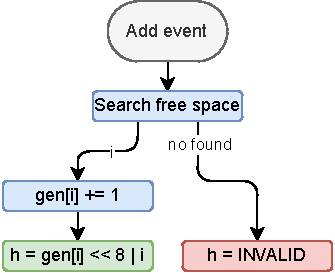
\includegraphics[width=0.6\textwidth]{figures/elec/led_sched_add_event.drawio.pdf}
	\caption{Délivrance d'un identifiant à l'ajout d'un événement}
	\label{fig:led_sched_add_event}
	\end{figure}
\end{minipage}
\hfill\hfill

\newpage

\begin{minipage}{0.40\textwidth}
\vspace{-1cm}
La validation d'un identifiant consiste à en extraire l'indice de l'emplacement désigné, puis à vérifier que cet emplacement est
occupé et que sa génération coïncide avec celle encodée dans l'identifiant (figure~\ref{fig:led_sched_handle_valid}).\\

Le retrait et le test de validité reposent tous deux sur cette vérification.\\

Un identifiant dont l'événement a disparu devient ainsi inopérant sans que son détenteur ait à en être informé, et ne peut en
aucun cas affecter l'événement qui occupe désormais l'emplacement.
\end{minipage}
\hfill
\begin{minipage}{0.30\textwidth}
	\vspace{-1cm}
	\begin{figure}[H]
		\centering
		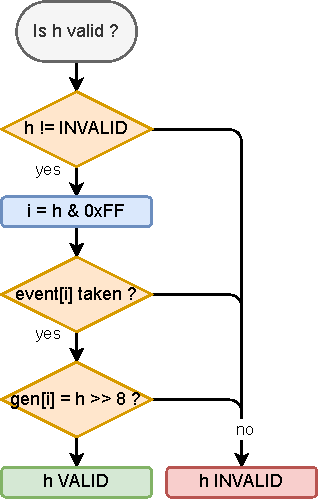
\includegraphics[width=0.8\textwidth]{figures/elec/led_sched_handler_valid.drawio.pdf}
		\caption{Validation d'un identifiant d'événement}
		\label{fig:led_sched_handle_valid}
	\end{figure}
\end{minipage}
\hfill\hfill

\subparagraph*{Résolution des événements : priorité et opacité} À chaque appel de \texttt{LedSched\_Process}, l'ordonnanceur
détermine, parmi les événements présents dans la pool, ceux dont la couleur contribue à l'affichage. Cette résolution repose
uniquement sur deux paramètres de chaque événement, sa priorité et son opacité, et s'effectue en deux passes sur la pool.

\hspace*{-\parindent}%
\begin{minipage}{0.5\textwidth}
\begin{figure}[H]
	\centering
	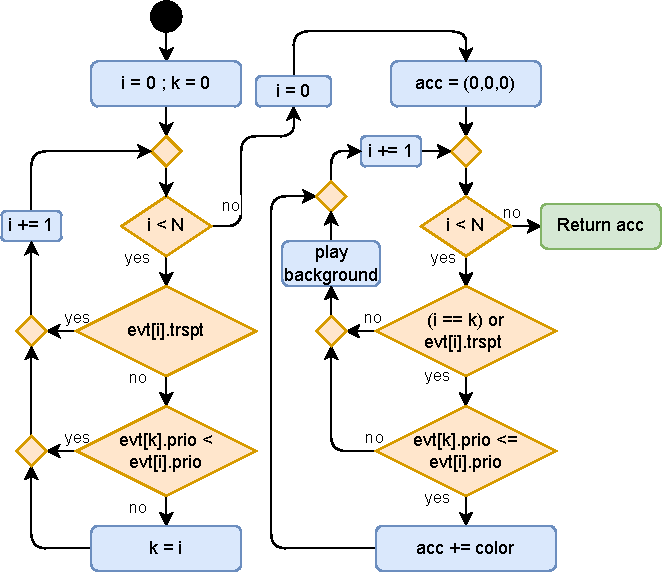
\includegraphics[width=\linewidth]{figures/elec/led_sched_process.drawio.pdf}
	\caption{Algorithme de résolution des événements}
	\label{fig:led_sched_resolution}
\end{figure}
\end{minipage}
\hfill
\begin{minipage}{0.48\textwidth}
La première passe élit un unique événement opaque : celui de plus haute priorité et, à priorité égale, le plus récemment ajouté.
La priorité de cet événement définit un seuil de visibilité pour l'ensemble de la pool. La seconde passe détermine le sort de
chaque événement. Sont joués l'opaque élu ainsi que tous les événements transparents de priorité supérieure ou égale au seuil
En l'absence de tout événement opaque, l'ensemble des événements transparents est joué.\\

Les couleurs des événements joués sont additionnées canal par canal, chaque canal étant borné à 1. Tous les autres événements
sont masqués et ne contribuent pas à la couleur affichée. La figure~\ref{fig:led_sched_resolution} présente l'algorithme de
résolution correspondant.
\end{minipage}

\vspace{0.4cm}

Les paramètres de priorité et d'opacité suffisent à exprimer plusieurs modes de cohabitation entre événements, sans qu'aucune
coordination ne soit nécessaire entre les parties du programme qui les ajoutent :
\begin{itemize}
    \item \textbf{Exclusion} : des événements opaques de même priorité se remplacent mutuellement, le dernier ajouté étant le
	seul affiché.
    \item \textbf{Superposition} : des événements transparents de même niveau sont affichés simultanément. Lorsque leurs motifs
	occupent des portions disjointes d'une même période, chacun reste distinctement perceptible.
    \item \textbf{Masquage} : un événement opaque de priorité élevée recouvre l'ensemble des événements de priorité inférieure.
    \item \textbf{Surimpression} : un événement transparent de priorité supérieure à celle de l'opaque élu s'ajoute à sa couleur
	au lieu de la remplacer.
\end{itemize}

La résolution ne conserve aucun état d'une itération à l'autre : elle est intégralement recalculée à chaque appel à partir du
contenu du pool. Lorsqu'un événement masquant disparaît, les événements qu'il recouvrait redeviennent visibles dès l'itération
suivante, sans qu'aucune sauvegarde ni restauration de l'affichage précédent ne soit réalisée par le programme appelant.

\newpage

\paragraph{Exemple d'utilisation} Le code ci-dessous met en \oe uvre un scénario de trois événements, dont l'exécution est
représentée sur la figure~\ref{fig:led_sched_frise}. Les motifs A et B sont périodiques, de période 1~s, et consistent
respectivement en un créneau vert sur la première moitié de la période et en un créneau bleu sur la seconde moitié. Ils sont
ajoutés comme événements transparents de même priorité, et ne diffèrent que par leur délai de pause : infini pour A et de 1~s
pour B. Le motif C, non périodique et d'une durée de 2,5~s, consiste en une bosse sinusoïdale rouge. Il est ajouté comme
événement opaque de priorité supérieure.

\vfill

\begin{lstlisting}[language=C, frame=tb, basicstyle=\small]
static waveform_space_t wave_a, wave_b, wave_c;

static waveform_space_mult_const_t ctx_a = {
    .wave_function_mult = waveform_gate,
    .ctx_mult = &(const waveform_gate_t) {
        .start = 0.0f, .end = 0.5f
    },
    .factor = (float3_t){ .x = 0.0f, .y = 1.0f, .z = 0.0f }
};

static waveform_space_mult_const_t ctx_b = {
    .wave_function_mult = waveform_gate,
    .ctx_mult = &(const waveform_gate_t) {
        .start = 0.5f, .end = 1.0f
    },
    .factor = (float3_t){ .x = 0.0f, .y = 0.0f, .z = 1.0f }
};

static waveform_space_mult_const_t ctx_c = {
    .wave_function_mult = waveform_sine,
    .ctx_mult = &(const waveform_sine_t) {
        .start = 0.0f, .end = 1.0f
    },
    .factor = (float3_t){ .x = 1.0f, .y = 0.0f, .z = 0.0f }
};

static led_evt_handle_t h_a = LED_SCHED_HANDLE_INVALID;
static led_evt_handle_t h_b = LED_SCHED_HANDLE_INVALID;
static led_evt_handle_t h_c = LED_SCHED_HANDLE_INVALID;

void setup() {
    Waveform_Init_Space(&wave_a, waveform_space_mult_const, &ctx_a, 1000, true);
    Waveform_Init_Space(&wave_b, waveform_space_mult_const, &ctx_b, 1000, true);
    Waveform_Init_Space(&wave_c, waveform_space_mult_const, &ctx_c, 2500, false);

    LedSched_Init();
    h_a = LedSched_Add(&wave_a, 0, true, HAL_MAX_DELAY, LED_SCHED_NO_FORCE);
    h_b = LedSched_Add(&wave_b, 0, true, 1000, LED_SCHED_NO_FORCE);
}

void loop() {
    uint32_t now = HAL_GetTick();
    if (!Led_Sched_IsValid(h_c) && now >= 3000) {
        h_c = LedSched_Add(&wave_c, 1, false, 0, LED_SCHED_NO_FORCE);
    }
    if (Led_Sched_IsValid(h_a) && now >= 7000) {
        LedSched_Remove(h_a);
    }
    LED_RGB_SetColor(&led_rgb, LedSched_Process(now));
}
\end{lstlisting}

\vfill\vfill

\newpage

\begin{itemize}
	\item De 0 à 3~s, A et B sont joués simultanément : leurs motifs occupant des portions disjointes de la période, la LED
	alterne entre le vert et le bleu.\\

	\item L'ajout de C à 3~s masque les deux événements transparents, qui sont mis en pause, et seul C est affiché.\\

	\item À 4~s, le délai de pause de B expire : B poursuit alors son exécution sans être affiché, tandis que A reste en pause.\\

	\item À 5,5~s, C se termine et libère son emplacement. A et B redeviennent visibles et dans la même phase.\\

	\item À 7~s, A est retiré de la pool et B reste seul affiché.
\end{itemize}

\begin{figure}[H]
\centering
% ================== Paramètres du scénario (s) ==================
\pgfmathsetmacro{\Per}{1}        % période des motifs A et B
\pgfmathsetmacro{\TaddC}{3}      % ajout de C
\pgfmathsetmacro{\DurC}{2.5}     % durée de C
\pgfmathsetmacro{\PauseB}{1}     % délai de pause de B
\pgfmathsetmacro{\TremA}{7}      % retrait de A
\pgfmathtruncatemacro{\Tend}{10} % fin de la frise (entier)
% ---- grandeurs dérivées ----
\pgfmathsetmacro{\TfinC}{\TaddC+\DurC}
\pgfmathsetmacro{\OffA}{\DurC}                % A : pause illimitée
\pgfmathsetmacro{\OffB}{min(\PauseB,\DurC)}   % B : pause bornée par son délai
\pgfmathsetmacro{\TfinPB}{\TaddC+\OffB}
% ================== Paramètres graphiques ==================
\def\Xs{1.2}      % cm par seconde
\def\LaneH{1.1}   % hauteur d'une ligne
\def\Amp{0.7}     % amplitude des courbes
\def\Nstrip{400}  % échantillons du bandeau
% ================== Motifs ==================
\pgfmathdeclarefunction{fr}{1}{\pgfmathparse{#1-floor(#1)}}
\pgfmathdeclarefunction{gA}{1}{\pgfmathparse{ifthenelse(fr((#1)/\Per)<0.5,1,0)}}
\pgfmathdeclarefunction{gB}{1}{\pgfmathparse{ifthenelse(fr((#1)/\Per)>=0.5,1,0)}}
\pgfmathdeclarefunction{bC}{1}{\pgfmathparse{0.5-0.5*cos(360*((#1)-\TaddC)/\DurC)}}
% couleur affichée
\pgfmathdeclarefunction{ledR}{1}{\pgfmathparse{ifthenelse((#1>=\TaddC)&&(#1<\TfinC), bC(#1), 0)}}
\pgfmathdeclarefunction{ledG}{1}{\pgfmathparse{ifthenelse(#1<\TaddC, gA(#1), ifthenelse((#1>=\TfinC)&&(#1<\TremA), gA(#1-\OffA), 0))}}
\pgfmathdeclarefunction{ledB}{1}{\pgfmathparse{ifthenelse(#1<\TaddC, gB(#1), ifthenelse(#1>=\TfinC, gB(#1-\OffB), 0))}}

\begin{tikzpicture}[x=\Xs cm, y=1cm,
  lane/.style={draw=black!25},
  played/.style={thick},
  silent/.style={thick, dashed, opacity=0.35},
  paused/.style={pattern=north east lines, pattern color=black!40},
  evt/.style={densely dashed, black!60}]

  \foreach \k/\name in {0/A, 1/B, 2/C}{
    \draw[lane] (0,-\k*\LaneH) -- (\Tend,-\k*\LaneH);
    \node[anchor=east] at (-0.1,{-\k*\LaneH+0.35}) {\name};
  }
  \pgfmathsetmacro{\yA}{0}
  \pgfmathsetmacro{\yB}{-\LaneH}
  \pgfmathsetmacro{\yC}{-2*\LaneH}
  \pgfmathsetmacro{\yL}{-3*\LaneH}

  % ---- A : joué, pause (illimitée), joué déphasé, retiré ----
  \draw[played, green!60!black] plot[domain=0:\TaddC, samples=241] (\x,{\yA+\Amp*gA(\x)});
  \fill[paused] (\TaddC,\yA) rectangle (\TfinC,\yA+\Amp);
  \node[font=\scriptsize, fill=white, inner sep=1pt] at ({(\TaddC+\TfinC)/2},{\yA+\Amp/2}) {pause};
  \draw[played, green!60!black] plot[domain=\TfinC:\TremA, samples=201] (\x,{\yA+\Amp*gA(\x-\OffA)});

  % ---- B : joué, pause, exécution silencieuse, joué ----
  \draw[played, blue] plot[domain=0:\TaddC, samples=241] (\x,{\yB+\Amp*gB(\x)});
  \fill[paused] (\TaddC,\yB) rectangle (\TfinPB,\yB+\Amp);
  \node[font=\scriptsize, fill=white, inner sep=1pt] at ({(\TaddC+\TfinPB)/2},{\yB+\Amp/2}) {pause};
  \pgfmathparse{\OffB<\DurC}
  \ifnum\pgfmathresult=1
    \draw[silent, blue] plot[domain=\TfinPB:\TfinC, samples=121] (\x,{\yB+\Amp*gB(\x-\OffB)});
  \fi
  \draw[played, blue] plot[domain=\TfinC:\Tend, samples=441] (\x,{\yB+\Amp*gB(\x-\OffB)});

  % ---- C : joué puis terminé ----
  \draw[played, red] plot[domain=\TaddC:\TfinC, samples=81] (\x,{\yC+\Amp*bC(\x)});

  % ---- bandeau de la couleur affichée ----
  \node[anchor=east] at (-0.1,{\yL+0.3}) {LED};
  \pgfmathsetmacro{\dt}{\Tend/\Nstrip}
  \pgfmathtruncatemacro{\Nlast}{\Nstrip-1}
  \foreach \i in {0,...,\Nlast}{
    \pgfmathsetmacro{\t}{(\i+0.5)*\dt}
    \pgfmathsetmacro{\r}{ledR(\t)}
    \pgfmathsetmacro{\g}{ledG(\t)}
    \pgfmathsetmacro{\b}{ledB(\t)}
    \definecolor{ledc}{rgb}{\r,\g,\b}
    \fill[ledc] ({\i*\dt},\yL) rectangle ({(\i+1)*\dt+0.004},\yL+0.6);
  }
  \draw (0,\yL) rectangle (\Tend,\yL+0.6);

  % ---- instants des appels ----
  \foreach \t/\lab in {0/{ajout A, B}, \TaddC/{ajout C}, \TfinC/{fin de C}, \TremA/{retrait A}}{
    \draw[evt] (\t,\yL) -- (\t,\Amp+0.3);
    \node[font=\scriptsize, above] at (\t,\Amp+0.3) {\lab};
  }

  % ---- axe temporel ----
  \draw[->] (0,\yL-0.25) -- (\Tend+0.3,\yL-0.25) node[right] {$t$ (s)};
  \foreach \s in {0,...,\Tend}{
    \draw (\s,\yL-0.3) -- (\s,\yL-0.2);
    \node[font=\scriptsize, below] at (\s,\yL-0.3) {\s};
  }
\end{tikzpicture}
\caption{Exécution du scénario \texttt{led\_sched}. Trait plein : événement joué ; trait pointillé transparent : exécution silencieuse ; hachures : pause. Le bandeau inférieur représente la couleur affichée par la LED.}
\label{fig:led_sched_frise}
\end{figure}

\newpage
